\chapter{双重网络外部性下移动数据服务提供商收益最大化研究}

\textbf{本章摘要:} 
%移动社交网络极大地增强了人们的在线社交互动,产生了海量的移动数据流量,为无线服务提供商带来了可观的收入。然而,潜在的收入增长正面临着通信基础设施网络容量的限制,以及服务提供商之间竞争的影响。
本章研究了竞争性数据服务市场中多个服务提供商的定价策略,其中移动用户的数据消费行为受到两方面因素的影响:社交效应(正网络外部性)和拥塞效应(负网络外部性)。为了分析移动用户和服务提供商之间的策略互动,本文设计了一个两阶段的斯塔克伯格博弈,分别由第一阶段的提供商博弈和第二阶段的用户博弈组成。针对用户博弈,本章刻画了均衡解的特征并建立了它的唯一存在性。对于提供商博弈,本章的分析表明,在提供商行为理性的场景以及提供商行为有限理性的场景下,混合策略均衡解的存在性都是有所保证的。进一步,本章提出了一种分布式学习算法,用于寻找混合策略均衡解决方案。本章第6节的的数值仿真结果对于社交效应和拥塞效应如何影响系统性能提出了见解,并验证了提供商有限理性行为为其收益带来的损失。

%Mobile social networks have greatly strengthened people's online social interactions, generating massive volume of mobile data traffic, and bringing remarkable revenues to the wireless service providers. Meanwhile, the potential revenue growth is restrained by the network capacity of physical communication infrastructure, and also challenged by the competition among service providers themselves. In this paper, we study the pricing strategies of multiple service providers in a competitive data service market, where mobile users' data consumption behaviors are influenced by two effects: the positive network effect and the congestion effect. To analyze the strategic interactions between mobile users and service providers, we device a two-stage Stackelberg game consisting a pricing game in Stage I and a usage game in Stage II, respectively. In particular, for the usage game, we characterize the equilibrium solution and establish its uniqueness. For the pricing game, our analysis indicates that a mixed-strategy equilibrium solution is guaranteed for the scenario with rational providers as well as the scenario with providers of bounded rationality. We further develop a distributed learning algorithm for finding a mixed-strategy equilibrium solution in the second scenario. Our numerical results provide insights into how positive network effect and congestion effect would impact the system performance, and demonstrate that the bounded rational behavior incurs degradation to service providers' revenues.

\textbf{关键词:}移动社交网络;网络定价;网络外部性;博弈论;展望理论
%\keywords{多目标跟踪;实时性;整数规划}

\section{引言}

在过去的十年中,人们对于移动智能设备的使用量经历了巨大的增长。对于不同背景和年龄的人群,移动智能设备如今已然成为他们日常生活中不可或缺的一部分。近年来,智能设备的普及也同时给在线社交网络(例如Facebook \cite{FB},Twitter \cite{Twitter})带来了巨大成功,极大地促进了人们的在线社交互动。统计数据显示,由于智能设备和在线社交网络的激增,全球移动社交用户数量早在2017年1月就已超过25亿,占社交媒体用户总数的91%\cite{Wearesocial}。
%The use of smart devices has experienced immense growth in the past decade, becoming an indispensable part of the daily life for most people around world, regardless of their backgrounds and age. In line with the pervasive penetration of smart devices, recent years have also witnessed the spectacular success of online social networks (e.g., Facebook\cite{FB}, Twitter\cite{Twitter}), which have greatly strengthened people's online social interactions.  Attributed to the proliferation of both smart devices and online social networks, the mobile social users has increased by 30\% year-over-year to surpass 2.5 billion globally in January 2017, accounting for 91\% of the total social media users \cite{Wearesocial}.

移动社交用户的激增不仅为社交网络平台带来了丰厚的利润,而且还为无线服务提供商带来了可观的收入。直观上,如今市场上众多经过精心设计的移动社交应用程序,使得人们可以随时随地与他们现有的朋友或未曾相似的用户进行在线互动(通过互发信息,多媒体共享和在线游戏等方式)。在这种{\kaishu 正网络外部性}作用\cite{David10}下,用户间社交关系的增强与扩展会反过来激发更多数据流量消费。例如,市场调研结果表明,如果某个手机游戏在一个用户的社交好友圈中非常受欢迎,那么该用户通常也会更喜欢玩该游戏。心理学上对这种潜在影响的分析为:个体通常希望自己可以被视为同伴中的一部分。这种正网络外部性可以在整个移动社交网络中广泛传播,从而导致数据使用量整体激增,为无线提供商带来可观的潜在收入。
%The explosion of mobile social users not only brings remarkable profit to the social network platforms, but also delivers great revenues to the wireless service providers. Intuitively, mobile social applications are well-designed nowadays to encourage peopzule's online interaction with either their known friends or other unacquainted users anytime and anywhere (e.g., via messaging, media sharing, and online gaming, etc.). The strengthened and expanded social relationship will in turn give rise to greater data consumption owing to {\em positive network effect}\footnote{The network effect is a concept in economic and business describing that the value of a good or service to one user is influenced by others' valuation on that good or service. A positive network effect normally refers to the phenomenon whereby a product or service becomes more valuable as more people accept it, encouraging ever-increasing numbers of users.\\}\cite{David10}. For instance, a user usually becomes more involved into playing a mobile game if that game has gained much popularity among her social friends. A psychological explanation of this effect is that users always want to be perceived as part of their peers.
%As another example, a user online video-streaming, her social friends are playing the same mobile gameher friendsor watching an online streaming video if her social friends areor the public, even if she is not quite interested into it at the beginning. 
%Such kind of positive network effect could be conveyed extensively throughout the mobile social network, resulting a fire-up of data consumption that has potential to generate significant revenues for the wireless providers. 
然而与此同时,无线通信网络的有限容量已逐渐成为正网络外部性下流量增长的主要制约。以在线手机游戏平台为例,由于无线通信带宽有限,在每天高峰时间段,活跃用户数量的增加以及所产生的累积数据流量时常导致数据传输的拥塞与服务的延迟。这种{\kaishu 负网络外部性}效应下用户体验上的影响将降低那些对延迟较为敏感的用户的活跃度,给服务提供商带来收入上的损失。
%However, with increasingly many on-the-shelf mobile applications being data-hungry, the potential growth of providers' revenues from network effect is constrained by the capacity of wireless communication network. Take the online mobile game platform as an example, the increasing number of active users at the peak time and the generated accumulated data traffic will result in serious congestion (hence service delays) due to limited bandwidth. And the resulted bad user experience would discourage users' data usage in such kind of delay-sensitive applications, which brings revenue loss to service providers.

使用合理的定价机制是一种重要的网络流量调控手段。传统通信网络中的定价问题已经在文献\cite{Walrand08,Huang10,Xinbin,CaoTVT,Xiaoming}中得到了较好的解决。对于移动无线通信网络中的定价问题,一些研究工作也已经将用户数据使用行为所受到的正网络外部性影响考虑进来\cite{Hartline08,Candogan12,SwapnaES12}。
近期,Gong等\cite{GongDCZ17}对单一服务提供商的无线数据服务市场中移动用户在网络效应和拥塞效应下数据消费行为进行了研究。然而在一些现实场景中,移动用户已经不再局限于单个服务提供商,而是可以选择从多个无线服务提供商购买服务\footnote{例如,在美国,移动用户可以通过订阅例如Google的Project Fi \cite{GoogleFi}这样的虚拟网络运营商来使用T-mobile和Sprint的数据服务。}。另一方面,实际中的一些迹象表明个体决策通常会偏离期望效用理论(Expected Utility Theory)框架\cite{Von}所预期的理性决策。在行为经济学领域进行的一些现有研究工作\cite{camerer2011behavioral}指出,个体的非理性行为时常归因于以下事实:当面对竞争和不确定性时,不同的个体会对他们的风险和收益进行不同且主观的评估。基于以上的观察与发现,本章考虑了多个服务提供商策略性争夺无线服务市场份额的问题场景,研究了在双重网络外部性效应下服务提供商以最大化其业务收益为目标的定价机制设计问题,并在建模中对于提供商的一些非完全理性行为进行了充分的考量。

%以上这些发现,使得对无线服务商寡头市场中定价决策的研究变得尤为有意义。
%Recently, the authors in\cite{GongDCZ17} have investigated the mobile users' data consumption behavior under both the network effect and the congestion effect in a single wireless service provider market. Meanwhile, instead of being restricted to a single service provider, mobile users nowadays have had the option to purchase services from multiple wireless service providers\footnote{For example, mobile users can subscribe to the service of both T-mobile and Sprint via virtual network operator such as Google's Project Fi \cite{GoogleFi}.}. Motivated by this observation, this study considers a scenario where multiple service providers need to compete strategically for the shares of the wireless service market to maximize their business revenues. Another observation inspiring this study is that individuals' decision making in reality usually deviate from the rational ones expected according to the well-established Expected Utility Theory framework \cite{Von}. Some existing research works done within the field of behavior economics \cite{camerer2011behavioral} have indicated that the irrationality is attributed to the fact that different individuals would have different and subjective evaluations on their risks and revenues when facing with competitions and uncertainties in practice.
%In order to optimize their utilities, the mobile users thereby need to strategically determine their data consumption from each of the service providers, with consideration of the social influence and congestion effect. On the other side, multiple service providers have to compete against each other for mobile users by adjusting their service prices in order to maximize their revenues in the market. Further, 
%With all these insights, it is of great interest to study the pricing-usage decision interaction in an oligopoly market of multiple wireless service providers.

简而言之,本章研究了一个具有多个服务提供商的竞争型无线数据服务市场,其中移动用户在确定其数据使用量时同时考虑两方面因素的影响,即对应于正网络外部性的社交效应以及对应于负网络外部性的拥塞效应。本文使用斯塔克伯格(Stackelberg)博弈\cite{osborne}的模型将提供商定价问题与用户数据使用问题结合起来进行建模。当博弈中服务提供商和个人用户的策略行为达到均衡状态时,任何独立的个体无法通过改变其策略获得更好的自身效用。对于刻画用户博弈均衡时的一个挑战在于每个用户的策略空间为多维空间(每个用户可以同时选用多个服务提供商的数据服务)。为了应对这一挑战,本文将连接任一用户和任一提供商的链接视为一个“虚拟用户”,并相应地对于每个“虚拟用户”的数据使用量进行考量。具体来说,在博弈的第一阶段,提供商会审慎地对其数据服务的单价进行设置以最大程度提高其潜在收益。在博弈的第二阶段中,给定每个提供商的单位数据服务价格,每个“虚拟用户”会策略性地确定其数据使用量,以优化其自身所获得的效用。在满足一定条件时,“虚拟用户”之间博弈均衡解的存在性以及唯一性可以被证明。在此基础上,可以进一步证明提供商定价博弈中$\epsilon$-混合策略价格均衡的存在性。
%In a nut shell, this paper studies a wireless service market with multiple competitive service providers, and a group of data consuming mobile users that strategically determine their data usage subject to the two different effects, namely positive network effect and congestion effect. To this end, we formulate the pricing-usage problem as a \emph{Stackelberg game}\cite{osborne}, in which service providers and individual users determine their strategies aiming to get to an equilibrium state, where no one could be better off by unilaterally deviate from the equilibrium point. One key challenge in characterizing the game lies in the high dimensionality of each user's strategy space. To tackle this challenge, we treat each link connecting one user and one provider as a ``virtual user'', and quantify the data usage of each ``virtual user'' accordingly. Specifically, in Stage I of the game, providers deliberately set the unit price of their data service in order to maximize her potential revenue. In Stage II, each ``virtual user'' determines her data usage strategically to optimize the corresponding payoff, given the service price of each provider. Under some technical conditions, we show both the existence and uniqueness of the equilibrium solution among ``virtual users'', based on which, we further show the existence of an $\epsilon$-mixed-strategy pricing equilibrium for the providers.

为了描述有限理性提供者的定价决策行为,本章第5节应用{\kaishu 展望理论}\cite{Kahneman}对第一阶段提供商之间的定价博弈作了进一步分析研究。作为诺贝尔经济学奖获奖理论,展望理论被用以模拟和解释存在风险和不确定性下的个人决策\cite{Tianming,Yu},并已被应用于一些实际问题场景中。例如,Li等\cite{Tianming}研究了一种无线环境下的随机接入博弈,其中用户考虑了展望理论中的{\kaishu 概率失真效应}作用,策略性地确定其在冲突信道上的传输概率。
%Yu等\cite{Yu}研究了一种数据市场模型,模型中用户需要选择成为数据卖方还是数据买方,并确定交易的数据量。他们考虑了展望理论中的{\kaishu 概率失真效应}和{\kaishu 效用框架效应}对用户决策行为的影响,并将该问题表述为非凸优化问题。
本章同时考虑了展望理论所涉及的两个主要现象:{\kaishu 概率失真效应}和{\kaishu 效用框架效应}。本章的分析表明,在这两种效应影响下​​,给定一定条件,$\epsilon$-混合策略定价均衡仍然存在。由于这种情况下服务提供商的收益函数不再被假设为已知信息,本文诉诸于分布式学习算法,使得服务提供商通过观察到的部分信息可以学习得到$\epsilon$-混合策略的定价均衡。数值结果表明,提供商的有限理性行为最终会导致其期望收入的下降。
%In order to characterize the pricing behaviors of bounded rational providers, we further study the pricing game in Stage II by appealing to \emph{Prospect Theory}\cite{Kahneman}. This Nobel-prize-winning theory has been utilized in several real-life applications to model and explain individuals' decisions under risks and uncertainty \cite{Tianming, Yu}. In this study, we particularly consider two main aspects of Prospect Theory: the \emph{probability distortion effect} and the \emph{utility framing effect}. We show that the existence of an $\epsilon$-mixed-strategy pricing equilibrium still holds under the two effects given a mild condition. Since service providers' payoffs are no longer public information, we resort to a distributed learning algorithm, by which service providers with partial observation can learn to play out an $\epsilon$-mixed-strategy pricing equilibrium. Through numerical results, we show that the expected revenue of provider suffers from a degradation as a result of providers' bounded rational behaviors.

本章的剩余部分组织如下。第\ref{sec:tvtmodel}节描述了无线服务提供商和移动用户之间的两阶段斯塔克伯格博弈的基本建模。第\ref{sec:stageII}节研究了针对用户之间流量使用的用户博弈,并描述了博弈的联边需求均衡解。第\ref{sec:stageI}节对提供商之间的定价博弈进行讨论和分析。最后,第\ref{sec:stageI2}节从展望理论的角度重新审视了服务提供商之间的定价博弈问题。相关的数值仿真结果在第\ref{sec:sim}节中给出,第\ref{sec:tvtcon}节对本章进行了总结。
%The remainder of the paper is organized as follows. We first discuss the related work in Section \ref{sec:related}. In Section \ref{sec:model}, we describe the basic formulation of the two-stage Stackelberg game between wireless service providers and mobile users. In Section \ref{sec:stageII}, we study the usage game among mobile users and characterize the link demand equilibrium of the game. Then we study the pricing game among providers in Section \ref{sec:stageI}, followed by the Section \ref{sec:stageI2} which revisits the pricing game by appealing to Prospect Theory. Numerical results are given in Section \ref{sec:sim}, and Section \ref{sec:con} concludes the paper.

%\section{研究现状}\label{sec:tvtrelated}
%
%在通信网络中,当流量负载增加到超出基础架构的物理性质确定的容量时,就会发生拥塞。拥塞效应在一些数据速率较低的通信场景(例如\cite{Jiming}和\cite{Deng})中的影响可能并不突出。然而它的影响在许多数据通信速率较高的系统中变得尤为显著,目前已有相关文献对其做了进行了深入的研究(参见\cite{Asuman07,Fang09,Tran12}及其中的参考文献)。
%%In communication networks, congestion occurs as traffic load increases beyond the capacity determined by the physical nature of the infrastructure. The impact of congestion effect might not be prominence in some low-data-rate communication schemes (e.g., \cite{Jiming} and \cite{Deng}). While it is much more significant in many high-data-rate communication systems and has been studied extensively in related literatures (see, e.g. \cite{Asuman07,Fang09,Tran12} and the references therein). 
%
%近年来,移动网络的社交影响引起了服务提供商以及平台开发人员的广泛关注。如今,越来越多的移动用户通过在线社交网络(例如Facebook \cite{FB},Twitter\cite{Twitter})进行联络,用户的影响力和信息传播速度比以往任何时候都快\cite{Niyato}。在\cite{David10}中,作者将用户之间的社交效应建模为一种正面的网络效应。在\cite{Baochun}中,作者采用了类似的想法来刻画众包系统中不断增长的社交用户数量所带来的内在收益的增长,及其对于平台所应提供的部分外在奖励的节省。在\cite{social}中,为了减少峰值蜂窝负载,作者提出了一系列算法根据用户在社交网络中的位置选择出特定用户,并将内容主动地推送给这些用户。
%%In recent years, the social aspect of mobile networking has attracted much attention of service providers and also platform developers. As more and more mobile users are nowadays connected by online social networks (e.g., Facebook \cite{FB}, Twitter \cite{Twitter}), both the influences and information of users can propagate within the crowds faster than ever \cite{Niyato}. In \cite{David10}, the social effect among users has been modeled as a kind of positive network effect. In \cite{Baochun}, similar idea was adopted to characterize the effect that growing population of socially connected users in crowdsourcing system results in more intrinsic rewards, which helps save a part of extrinsic rewards that are supposed to be provided by the platform. In \cite{social}, in order to reduce the peak cellular load, the authors proposed a family of algorithms that proactively push content to particular users that are selected based on their positions in the social network. 
%
%在另外一些研究工作中,个体间的社交影响已经被用在解决许多网络设计和优化问题中。Chen等\cite{Chen13}利用社交信任和互惠互利因素,通过将问题转化为联盟博弈来改进D2D合作通信。XX等人则利用用户之间的社交距离进行用户关联,以增强具有底层D2D通信的小型蜂窝网络的系统性能\cite{Ashraf}。Yang等\cite{Guang}提出了一种移动群智感知系统设计,利用移动用户之间的社交联系来激励他们的参与和合作,以获取更高的回报。Chen等\cite{Chen14}提出了一个社交团体效用最大化(SGUM)框架,其中每个用户关注的是由自己的个人效用与社交朋友的效用所组成的“团体效用”。
%%Along another line of literatures, social influences among individuals have been utilized in solving many network design and optimization problems. In \cite{Chen13}, Chen \emph{et al.} have leveraged social trust and social reciprocity to enhance cooperative D2D communication by casting the problem to a coalitional game. In\cite{Ashraf}, the social distances between user equipments were exploited for the user association to enhance the system performance of a small cell network with underlaid D2D communication. 
%%In \cite{Huang17}, Cheung \emph{et al.} proposed a socially-aware reward mechanism for mobile crowdsensing system, where the platform exploits users' social relationship for profit maximization. 
%%In \cite{Guang}, Yang \emph{et al.} proposed a mobile crowd sensing system design that leverages social ties among mobile users to incentivize their participation and global cooperation for higher payoffs. In \cite{Chen14}, the authors developed a social group utility maximization (SGUM) framework, in which each user cares about the ``group utility'' consisting of her own utility as well as her social friends' utilities.  
%
%通信网络中的定价问题已经在文献\cite{Walrand08,Huang10,Xinbin,CaoTVT,Xiaoming}中得到了较好的解决。在一些重点关注单个服务提供商定价策略的研究工作中,移动用户的数据使用行为所受到正面网络影响已经被考虑进来,如\cite{Hartline08,Candogan12,SwapnaES12}。而据我们所知,目前还很少有在研究网络服务定价问题中同时考虑到网络效应和拥塞效应的影响。最近,Gong等\cite{GongDCZ17}首先研究了垄断市场中单个服务提供商的定价策略,在该市场中,移动用户的数据使用行为会同时受到这两种影响。相比于上述工作中所考虑的垄断市场,我们的前期工作\cite{MYCISS16}研究了寡头市场环境下的定价问题,即存在多个服务提供商之间争夺移动用户的数据市场的竞争。
%%The pricing problem in communication networks has been addressed extensively in the literature \cite{Walrand08,Huang10,Xinbin,CaoTVT,Xiaoming}. There has been a line of works focusing on investigating the pricing strategies of a single service provider, with the mobile users' data usage behavior subject to positive network effect (see, e.g., \cite{Hartline08,Candogan12,SwapnaES12}). 
%%Hartline \emph{et al.} propose a basic ``Influence and Exploit Marketing'' strategy in \cite{Hartline08}, which takes into consideration of sequential purchases, where myopic consumers make their consumption decisions based on their neighboring consumers who have already bought the product. Candogan \emph{et al.} in \cite{Candogan12} consider a simultaneous consumption decision making model for rational agents embedded in a social network. They formulate the interactions between the monopolist and agents as a Stackelberg game with linear-quadratic utility function for the agents. 
%%To the best of our knowledge, very little works on network pricing have considered the impact of both network effect and congestion effect. 
%%\cite{Johari10} has studied users' behaviors, when they experience both network effect and congestion effect. However, it assumes that the network effect is the same for all users, which does not capture the fact that users experience different levels of network effect based on their diverse social ties as considered in this paper. 
%%The authors in \cite{GongDCZ17} first studied the pricing strategy of a single service provider in a monopoly market where mobile users' data usage behaviors are subject to both the two effects. In contrast to \cite{GongDCZ17}, our preliminary work \cite{MYCISS16} investigated the pricing problem in an oligopoly market setting, where multiple service providers compete against each other for mobile users' data consumption.
%
%近些年,人们在解决一些实际的无线网络中的决策问题时,采用了展望理论(Prospect Theory)\cite{Kahneman}对决策过程进行建模。 例如,Li等\cite{Tianming}研究了一种无线环境下的随机接入博弈,其中用户考虑了展望理论中的概率失真效应作用,策略性地确定其在冲突信道上的传输概率。Yu等\cite{Yu}研究了一种数据市场模型,模型中用户需要选择成为数据卖方还是数据买方,并确定交易的数据量。他们考虑了展望理论中概率失真效应和效用框架效应对用户决策行为的影响,并将该问题表述为非凸优化问题。
%%Recently, Prospect Theory \cite{Kahneman} has been employed to model the decision making process within wireless networks in practice. In \cite{Tianming}, Li \emph{et al.} studied a wireless random access game, where users strategically determine their transmission probabilities over a collision channel under the probability distortion effect of Prospect Theory. Yu \emph{et al.} in \cite{Yu} studied a data market model, where users need to choose to be a data seller or a data buyer, and also determine the amount of data being traded. They formulated the problem as a non-convex optimization problem considering both the probability distortion effect and the utility framing effect on users' decision behaviors. 
%
%在本文中,我们考虑了可能存在的服务提供商行为有限理性的情况。在这种更为一般性的背景下,我们证明了用户博弈的混合策略定价均衡的存在,并给出了均衡唯一的条件。我们的数值结果表明,服务提供商的有限理性行为会导致总收入下降。
%%虽然部分工作已在\cite{MYCISS16}中进行了介绍,但本文中已添加了主要结果的完整证明,以帮助读者更好地理解。
%%In this paper, we extend our discussion in preliminary work \cite{MYCISS16} to a broader scope by considering the case where service providers can be of bounded rationality. And in this more general setting, we show the existence of a mixed-strategy pricing equilibrium of a usage game, and establish the condition under which the equilibrium is unique. Our numerical result indicates that service providers' bounded rationality can lead to degradation on the total revenues. While part of this work has been presented in \cite{MYCISS16}, complete proofs for the main results have been added in this paper to facilitate readers' better understanding.

\section{社交关系影响下移动数据的价格竞争}\label{sec:tvtmodel}

在本节中,我们首先提出了无线数据服务的寡头市场模型,在该模型中,互相之间具有社交关系的移动用户可以从一组服务提供商那里购买和使用数据服务。我们使用两阶段的\emph{斯塔克伯格博弈}对提供商和用户之间的交互进行建模。我们接下来对建模进行具体介绍。
%In this section, we first provide the oligopoly market model for the wireless data service, in which a crowd of socially connected mobile users can purchase and consume the data service from a group of service providers. We next describe the two-stage \emph{Stackelberg game} formulation that models the interactions between providers and users. 

%To tackle the challenge in characterizing the game in Stage II due to the multidimensional strategy space of each user, the data usage problem among users is cast as a game played by virtual players.

%\subsection{Socially-aware Mobile Data Usage and Wireless Providers' Pricing Strategies}
\subsection{系统模型}

我们考虑一组移动用户$\N\triangleq\{1,\cdots,N\}$从一组无线服务提供商$\K\triangleq\{1,2,\cdots,K \} $那里购买使用具有可替代性的无线数据服务\footnote{此处可替代性意味着使用来自不同服务提供商的等量数据对于用户来讲具有相同价值。}。每个用户可以从一个以上的服务提供商那里购买服务,其中用户$i$从服务提供商$k$消费的数据量(由$x^k_i$表示)。我们令$\mathbf{X}\in\mathbb{R}^{N\times K}$表示所有用户的使用情况,用$\mathbf{X}_{-i}$表示排除用户$i$后剩余用户的使用情况。
%Consider a set of mobile users $\N\triangleq\{1,\cdots,N\}$ consuming perfectly substitutable wireless services\footnote{Perfectly substitutable wireless services here means that the same amount of data usage from different service providers has the same valuation to a mobile user.} from a set of wireless service providers $\K\triangleq\{1,2,\cdots,K\}$. Each user can subscribe to more than one service providers with the data consumed by user $i$ from service provider $k$ denoted by $x^k_i$.
%Consider a market with a set of wireless service providers $\K\triangleq\{1,2,\cdots,K\}$, who provide perfectly substitutable wireless services\footnote{The same amount of data usage from different service providers has the same valuation to each mobile user.} to a set of mobile users $\N\triangleq\{1,\cdots,N\}$. Each user $i\in\N$ can subscribe to all $K$ service providers and the data usage consumed from service provider $k\in\K$ is denoted by $x_i^k$. 
%We let $\mathbf{X}\in\mathbb{R}^{N\times K}$ denotes the usage profile of all the users, and $\mathbf{X}_{-i}$ denotes the joint usage profile without user $i$.

我们假定移动用户之间存在社交关联,并使用社交联系量$g_ {ij}\in[0,1]$来量化用户$j$对用户$i$的社交影响。而社交影响所引发的{\kaishu 正网络外部性}使得移动用户随着其社交朋友数据使用量的增加获得更多的效用。
%The mobile users are assumed to be socially connected, with the social impact of user $j$ on user $i$ quantified by a positive social tie $g_{ij}\in[0,1]$. The social impact induces \emph{positive network effect}, under which mobile users are inclined to experience more utility gain as the usages of their social friends increase.
%which can be modeled by the product term $g_{ij}x_{i}^{k}x_j^k$ as in \cite{GongDCZ17} and \cite{Candogan12}.
%Due to the fact that social services encourage mobile users to demand more data usage (i.e., the positive network effect), we model this effect by using a social tie $g_{ij}\in[0,1]$ to quantify the social influence from user $j$ to user $i$. As in \cite{GongDCZ17} and \cite{Candogan12}, the product $g_{ij}x_{i}^{k}x_j^k$ can capture that a user derives more utility by increasing her usage in social services, and the marginal gain of social utility increases as her social friends increase their usage. 
另一方面,随着用户整体数据消耗的增加,拥塞效应(例如,服务延迟现象)作为一种{\kaishu 负网络外部性}效应将变得尤为显著。由此,本章在建模时所需要明确地将每个移动用户的个人效用分成四部分:固有效用,数据使用成本,社交效应和拥塞效应。具体来说,给定每个提供商收取的单位服务价格,用户$i$的单个效用可以写为
%As data consumption increases, the congestion effect (e.g., service delays) will become prominent, and need to be explicitly considered in our model. To this end, the individual utility of each mobile user includes four parts: the intrinsic utility, the data usage cost, the network effect, and the congestion effect. Specifically, given the unit service price charged by each provider, the individual utility of user $i$ can be written as
\begin{align}\label{eq:userU}
%\small
u_i&(\mathbf{x}_i,\mathbf{X}_{-i},\mathbf{p})=\underbrace{a_i\sum_{k\in\K}x^k_i-\frac{1}{2}b_i(\sum_{k\in\K}x^k_i)^2}_{\text{固有效用}}-\underbrace{\sum_{k\in\K}p_kx^k_i}_{\text{数据使用成本}}\nonumber\\
&+\underbrace{\sum_{k\in\K}x^k_i\sum_{j\in\N}g_{ij}\sum_{m\in\K}x^m_j}_{\text{社交效应(正网络外部性)}}-\underbrace{\frac{c}{2}\sum_{k\in\K,x_i^k>0}(\sum_{j\in\N}x^k_j)^2}_{\text{拥塞效应(负网络外部性)}},
\end{align}
其中$\mathbf{x}_i = (x_i^1,x_i^2,\cdots,x_i^K)$表示用户$i$的使用情况,而$\mathbf{p} = (p_1,\cdots, p_K)$表示所有服务提供商的定价策略,其中$p_k$表示来自提供商$k\in\K$的数据服务单价。同工作\cite{GongDCZ17}和工作\cite{Candogan12}相同,我们采用了二次函数形式的内在效用函数,其对类型广泛的一些凹函数来说是很好的二阶近似。具体来说,$a_i>0$和$b_i>0$是两个内在系数,用于表征使用数据服务对于用户$i$的固有效用。双重网络外部性中的社交效应被建模为来自用户$i$的总数据需求量的线性函数,因而其边际效用取决于其社交好友的总数据使用量乘以对应社会联系的加权总和(即$\sum_{j\in\N}g_{ij}\sum_{m\in\K}x^m_j$)。而对于双重网络外部性中的拥塞效应,本文建模中假设用户从单个服务提供商处所受到的拥塞影响与该服务提供商的总数据流量的平方成正比,其中参数$c>0$用以刻画物理通信介质的状况。用户受到的总拥塞影响是其受到各服务提供商拥塞影响的总和。
%where $\mathbf{x}_i=(x_i^1,x_i^2,\cdots,x_i^K)$ denotes the usage profile of user $i$, and $\mathbf{p}=(p_1,\cdots,p_K)$ denotes the joint pricing profile of all the service providers where $p_k$ denoting the unit price of data service from provider $k\in\K$. Following \cite{GongDCZ17} and \cite{Candogan12}, we apply a quadratic form intrinsic utility function, which serves as a good second-order approximation for a broad class of concave utility functions. Specifically, $a_i>0$ and $b_i>0$ are two intrinsic coefficients that characterize user $i$'s intrinsic valuation of her data consumption. The network effect is modeled as a linear function of the total data demand from user $i$, so that her marginal utility depends on the aggregated data demand of her social friends weighted by the social tie weights (i.e., $\sum_{j\in\N}g_{ij}\sum_{m\in\K}x^m_j$). The congestion effect a user experiences from a single service provider is proportional to the square of total data traffic of that service provider, with parameter $c > 0$ models the condition of the physical communication medium. The total congestion effect a user experiences is the aggregated congestion effect from all service providers that she has connection with. 

对于每个服务提供商$k\in\K$,我们令$q_k$表示其单位服务成本,并将其收入$v_k$表示为其收到的总付款减去她产生的总服务成本,
%For each service provider $k\in\K$, we denote $q_k$ as her customized unit service cost, and model her revenue $v_k$ as the the total payment she received minus the total service cost she incurred,
%The revenue of each  provider is as the difference between the total payment received and the total service cost. Let $q_k$ denote the customized unit service cost of provider $k\in\K$. Her revenue can be written as
\begin{equation}\label{eq:SPrev}
  v_k=p_k\sum_{j\in\N}x^k_j-q_k\sum_{j\in\N}x^k_j,~~\forall k\in\K,
\end{equation}
其中$p_k$由提供商$k$通过从包含$M_k$个不同价格水平的离散价格空间$\mathcal{P}_k\triangleq\{p_k^1,p_k^2,\cdots,p_k^{M_k}\}$中选择一个值来确定。所有服务提供商的联合价格空间定义为$\mathcal{P}\triangleq\prod_ {k\in\K}\mathcal{P}_{k}$。图\ref{fg:scheme}展示了系统模型以及服务提供商和移动用户之间的交互关系。简单来说,服务提供商通过策略性地制定服务价格来争夺数据需求大的移动用户。而在给定提供商的服务定价后,自利的移动用户需要在社交效应和拥塞效应的影响下决定其数据使用情况。在下一部分中,我们将介绍问题的博弈论表述。
%where $p_k$ is determined by provider $k$ by choosing a value from her price space $\mathcal{P}_k\triangleq\{p_k^1,p_k^2,\cdots,p_k^{M_k}\}$, which consists of $M_k$ different price levels. The joint price space of all service providers is defined as $\mathcal{P}\triangleq\prod_{k\in\K}\mathcal{P}_{k}$. Fig. \ref{fg:scheme} illustrates the system model and the interactions among service providers and mobile users. Basically, the service providers compete for data demanding mobile users by strategically pricing their services; given the pricing profiles, the self-interested mobile users need to decide their data usage profile under the impacts of network effect and congestion effect. In the next section, we introduce the game theoretic formulation of the problem.
\begin{figure}[htb]
\centering
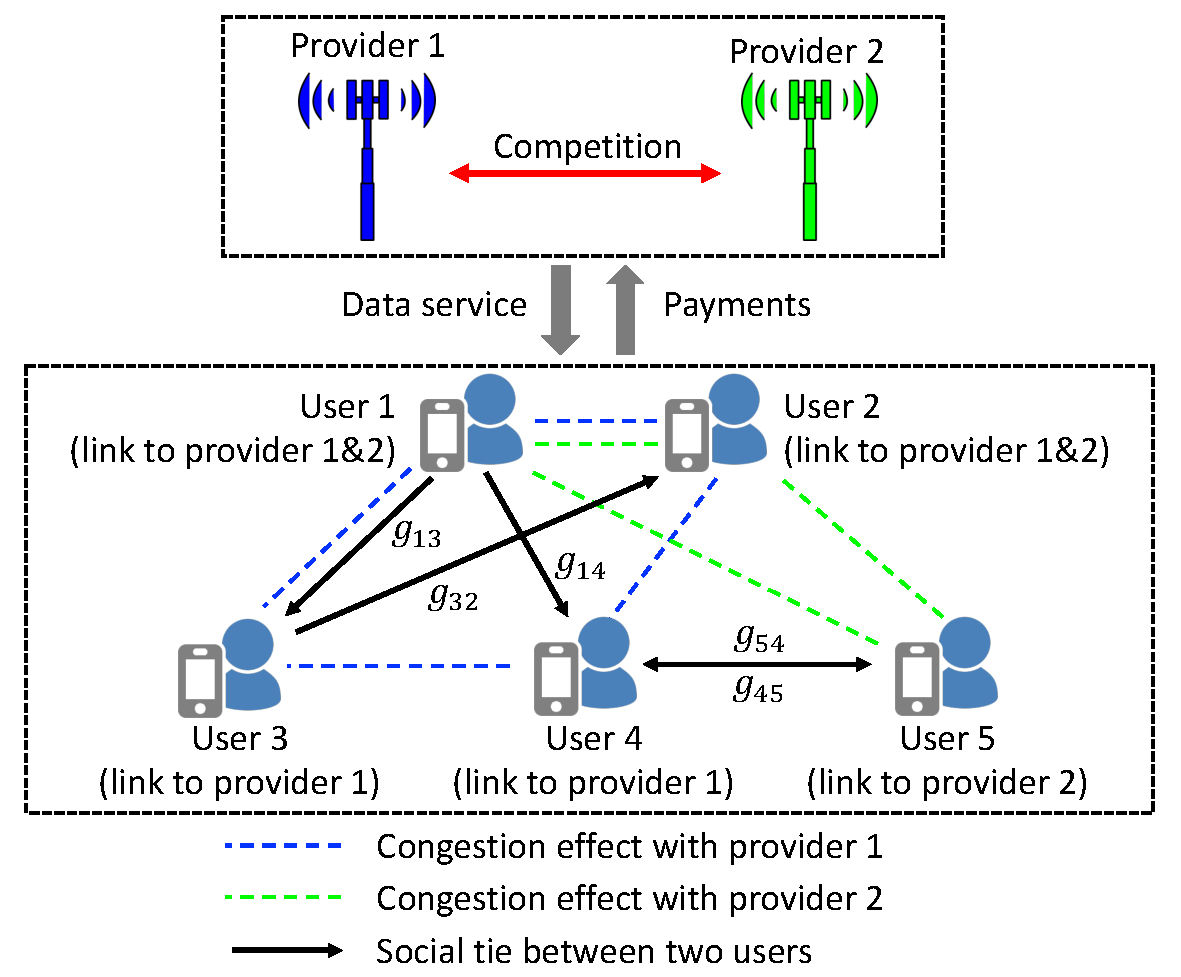
\includegraphics[scale=0.56]{./pic/scheme0.pdf}
\vspace{-0.0cm}
%\caption{An illustration of the system model and interactions among service providers and mobile users.}\label{fg:scheme}
\caption{系统模型以及服务提供商和移动用户之间的交互关系示意图。}\label{fg:scheme}
\end{figure}


\subsection{斯塔克伯格博弈建模}
在本节中,我们将提供商定价-用户数据使用的问题建模为一个两阶段的\emph{斯塔克伯格博弈}。服务提供商通过阶段\uppercase\expandafter{\romannumeral1}中的非合作博弈来确定其服务定价,而其定价策略是基于第二阶段子博弈中用户之间的子博弈所确定的。
%In this section, we cast the pricing-usage problem as a two-stage \emph{Stackelberg game} where service providers determine their pricing profiles via a non-cooperative game in stage I, based on the total data demands determined by mobile users via a subgame in stage II.
%The equilibrium of the game (if exists) would provide a satisfying solution in the sense that no one could be better off by unilaterally deviate from the equilibrium strategy.
%Specifically, in Stage I, given the pricing strategies of other providers, each provider determines the unit service price to maximize its revenue, and then announces the price to users. In Stage II, given the price from each  provider, each mobile user decides her data usage from each provider to maximize her individual utility. 
与文献[\citenum{GongDCZ17}]中考虑的垄断市场不同,在我们的案例中,每个移动用户的战略空间都是多维的,这给刻画用户博弈的均衡解增添了挑战。针对这一挑战,我们把联结一个移动用户和一个服务提供商的链接视为一个\emph{虚拟玩家},并将用户之间的数据使用问题视为虚拟玩家(链接)间的非合作博弈。我们令$\mathcal{L}\triangleq\{(i,k)\}_{i\in\N,k\in\K}$表示$L = N\times K$个链接的集合。虚拟玩家$(i,k)$的纯策略是指流经链接$(i,k)$的数据量$x^{k}_{i}$,而玩家$(i,k)$的收益对应于$u_{i}$(即始于同一用户的虚拟玩家具有相同的收益)。进而链接$(i',k')$对链接$(i,k)$的社交效应可以通过用户$i$和$i'$之间的社交联系量$g_{ii'}$来表征。我们令$\mathbf{x}=(\mathbf{x}_{1},\mathbf{x}_{2},\cdots,\mathbf{x}_{K})$表示所有链接上的数据使用量,并用$\mathbf{x}_{-(i,k)}$表示排除联结$(i,k)$后其他链接上的数据使用量。两阶段博弈的定义如下:
%Different from the monopoly market considered in \cite{GongDCZ17}, the strategy space of each mobile user in our case is multidimensional, making it more challenging to characterize the equilibrium of the usage game. To tackle this challenge, we treat the link connecting a mobile user and a provider as a \emph{virtual player}, and cast the data usage problem among users as a non-cooperative game played by virtual players (links). Let $\mathcal{L}\triangleq\{(i,k)\}_{i\in\N,k\in\K}$ denote the set of $L=N\times K$ user-provider links. The pure strategy of virtual player $(i,k)$ is the data usage $x^{k}_{i}$ over the link $(i,k)$ with its payoff corresponds to $u_{i}$ (i.e., the links starting from the same user have the same payoff). And it follows that the social network effect that link $(i',k')$ has on link $(i,k)$ can be characterized by the social tie $g_{ii'}$ between user $i$ and $i'$. We denote $\mathbf{x}=(\mathbf{x}_{1}, \mathbf{x}_{2},\cdots,\mathbf{x}_{K})$ as the joint link usage profile of all links, and use $\mathbf{x}_{-(i,k)}$ to denote the joint usage profile excluding $(i,k)$. And the two-stage game can be formally defined as follows:

\begin{df}[两阶段提供商定价-用户数据使用博弈]\label{def:mlmf}
\mbox{}
\begin{itemize}
    \item 阶段\uppercase\expandafter{\romannumeral1}(提供商定价博弈 $\mathcal{G}_P\triangleq\{\K,\mathcal{P},\{v_k\}_{k\in\K}\}$):\\
    在用户(链接)数据使用量为$\mathbf{x}$的情况下,给定其他提供商的定价策略$\mathbf{p}_{-k}$,每个提供商$k\in\K$选择$p_k$来最大化其收入$v_k$。定价博弈的均衡解可表示为一个联合定价策略$\mathbf{p}^*=(p^{*}_{1}\cdots,p^{*}_{K})$满足下式
    %Under the links' usage profile $\mathbf{x}$, each provider $k\in\K$ chooses $p_k$ to maximize its revenue $v_k$, given other providers' pricing strategies $\mathbf{p}_{-k}$. The pricing equilibrium is a joint pricing profile $\mathbf{p}^*=(p^{*}_{1}\cdots,p^{*}_{K})$ such that 
        \begin{equation}
          p^*_k=\arg\max_{p_k\in\mathcal{P}_k}v_k(p_k,\mathbf{p}^{*}_{-k},\mathbf{x}), ~\forall k\in\K.
        \end{equation}
        
    \item 阶段\uppercase\expandafter{\romannumeral2}(用户数据使用博弈$\mathcal{G}_U\triangleq\{\mathcal{L},\mathbb{R}_+^L,\{u_i\}_{i\in\N}\}$):\\
    给定提供商的定价策略$\mathbf{p}$和其他链接的数据使用量$\mathbf{x}_{-(i,k)}$,每个链接$(i,k)\in\mathcal{L}$选择从服务商$k$处使用量为$x^{k}_i$的服务以最大化其收益$u_ {i}$。用户数据使用博弈的均衡解可表示为$\mathbf{x^*}=(\mathbf{x}^*_{1},\mathbf{x}^*_{2},\cdots,\mathbf{x}^*_{K})$,这种情况下任何用户都无法通过单方面更改其使用量来增加其个人收益:
    %Given providers' pricing profile $\mathbf{p}$, each link $(i,k)\in\mathcal{L}$ chooses a usage demand $x^{k}_i$ to maximize her payoff $u_{i}$ given other links' usage profile $\mathbf{x}_{-(i,k)}$. The link demand equilibrium is a joint usage profile $\mathbf{x^*}=(\mathbf{x}^*_{1}, \mathbf{x}^*_{2},\cdots,\mathbf{x}^*_{K})$ such that no user can increase its payoff by unilaterally changing its usage profile:    
        \begin{equation}
          x^{k*}_i=\arg\max_{x^{k}_i\in \mathbb{R}_+}u_i(x^{k}_i,\mathbf{x}^*_{-(i,k)},\mathbf{p}), ~\forall i\in\N.
        \end{equation}
\end{itemize}
\end{df}

当博弈问题处于均衡解时任何参与博弈的玩家单方面偏离其均衡策略的行为都将导致其自身的收益降低。按照惯例,我们采用反向归纳法\cite{osborne}来分析斯塔克伯格博弈。我们首先来研究阶段\uppercase\expandafter{\romannumeral2}中的数据使用博弈。
%The equilibrium solution of the game (if exists) would provide a satisfying solution in the sense that any unilaterally deviation from the equilibrium solution would lead to a payoff degradation. By convention, we appeal to the backward induction approach\cite{osborne} to analyze the Stackelberg game. Next, we first study the usage game in Stage II. 



\section{用户数据使用博弈中的联结需求均衡}\label{sec:stageII}

在本节中,我们将在给定服务提供商定价策略的情况下研究提供商-用户链接的数据使用需求。根据公式(\ref{eq:userU})和一阶条件$\frac{\partial u_{i}}{\partial x^{k}_{i}} = 0$,我们获得了链接$(i,k)$的最佳响应函数为
%In this section, we study the usage demand over links given the joint pricing profile of service providers. Using function (\ref{eq:userU}) and the first-order condition, $\frac{\partial u_{i}}{\partial x^{k}_{i}}=0$, we obtain the best response function of link $(i,k)$ as
\begin{equation}\label{br1}
%\small
\bold{B}^{k}_{i}\left(\mathbf{x}_{-(i,k)}\right)=\max\left\{0,\frac{a_i-p_k}{b_i+c}-\frac{b_i\sum_{k'\neq k}x^{k'}_i}{b_i+c} + \frac{\sum_{j\neq i}g_{ij}\sum_{m\neq k}x_{j}^{m}}{b_i+c}+\frac{\sum_{j\neq i}(g_{ij}-c)x_{j}^{k}}{b_i+c}\right\}.
\end{equation}



根据(\ref{br1}),每个链接的最佳响应包括两部分:独立于其他链接的内在需求$\frac{a_i-p_k}{b_i + c}$,和取决于其他链接的外部需求$-\frac{b_i\sum_{k'\neq k}x^{k'}_i}{b_i + c} + \frac {\sum_{j\neq i}g_{ij}\sum_{m\neq k}x_{j}^{m}}{b_i + c} + \frac{\sum_{j\neq i}(g_{ij} -c)x_{j}^{k}}{b_i + c}$。具体来说,对于外部需求,第一项$-\frac{b_i \sum_{k'\neq k}x^{k'}_i}{b_i + c}$表征了其他同样始于用户$i$的链接对链接$(i,k)$的负面影响,这体现了使用除去提供商$k$以外的其他提供商的数据服务将削弱对于服务提供商$k$的数据使用。第二项$\frac{\sum_{j\neq i}g_{ij}\sum_{m\in\K}x_{j}^{m}}{b_i + c}$刻画了联结除用户$i$和提供商$k$的其他链接对于$(i,k)$所产生的正面网络外部性影响。第三项中的系数$\frac{g_{ij}-c}{b_i + c}$则刻画了与提供商$k$连接的其他链接对链接$(i,k)$上需求的边际影响。显然,如果社会效应主导了拥挤效应(即$g_{ij}\geq c$),则边际影响是正面的;而如果拥塞效应占主导地位(即$g_{ij} <c$),则边际影响为负面的。
%According to (\ref{br1}), the best response of each link consists of two parts: the internal demand, $\frac{a_i-p_k}{b_i+c}$, which is independent of other links, and the external demand, $-\frac{b_i\sum_{k'\neq k}x^{k'}_i}{b_i+c}+\frac{\sum_{j\neq i}g_{ij}\sum_{m\neq k}x_{j}^{m}}{b_i+c}+\frac{\sum_{j\neq i}(g_{ij}-c)x_{j}^{k}}{b_i+c}$, which depends on those links that are owned by the same user or are connected with the same service provider. Specifically, the first term $-\frac{b_i\sum_{k'\neq k}x^{k'}_i}{b_i+c}$ characterizes the negative effect on link $(i,k)$ from other links starting from user $i$, implying that the data usage from providers other than $k$ would dampen the usage from service provider $k$. The second term $\frac{\sum_{j\neq i}g_{ij}\sum_{m\in\K}x_{j}^{m}}{b_i+c}$ indicates the level of positive network effect on link $(i,k)$ from the links that connect user $i$'s social neighbors and service providers excluding $k$. The coefficient $\frac{g_{ij}-c}{b_i+c}$ characterizes the marginal impact on the demand of link $(i,k)$ from other links that also connect with provider $k$. Clearly, if the social effect dominates the congestion effect (i.e., $g_{ij}\geq c$), the marginal impact is positive; while if the congestion effect dominates (i.e., $g_{ij}<c$), the marginal impact is negative.

%\footnote{我们有$\forall i,i'\in\N$,如果$i<i'$,则\tau(i,k)<\tau(i',k)$;$\forall k,k'\in\K$,如果$k<k'$,则$\tau(i,k)<\tau(i,k')$。}


\subsection{联结需求均衡的存在性与唯一性}
我们首先讨论用户博弈中链接需求均衡的存在性。在不失一般性的前提下,我们仅关注数据使用量大于零的链接,而那些具有零使用量的链接在策略求解中是冗余的。令$\mathcal{L}^{+}$表示具有正数据使用量的链接集合,即$x^{k}_{i}> 0,\forall(i,k)\in\ca{L }^{+}$。我们定义$\tau:\ca{L}^{+}\rightarrow(1,2,\cdots,L^+)$为一个映射使得$\tau(i,k)$使用索引$l\in\{1,\cdots,L^+\}$\footnote{$\forall i,i'\in\N$,如果$i<i'$则$\tau(i,k)<\tau(i',k)$;$\forall k,k'\in\K$,如果$k<k'$,则$\tau(i,k)<\tau(i,k')$。}对链接$(i,k)\in\ca{L}^{+}$进行标记。为了方便起见,我们令$\mathbf{u}^+ =(u^{+}_{1},\cdots,u^{+}_{L^{+}})$表示效用向量,其中$u^{+}_{\tau(i,k)} = u_{i}$,$\mathbf{x}^{+} =(x^{+}_{1}, \cdots, x^{+}_{L^{+}})$表示使用向量,其中$x^{+}_{\tau(i,k)} = x^{k}_{i}$,$\mathbf{p}^+=(p^{+}_{1}, \cdots, p^{+}_{L^{+}})$表示价格向量,其中$p_{\tau(i,k)}^+ = p_k$表示链接$(i,k)$和$\mathbf{a}^+ =(a^{+}_{1}, \cdots, a^{+}_{L^{+}})$表示系数向量,其中$a_{\tau(i,k)}^+ = a_i$表示链接$(i,k)$的固有系数。我们通过图\ref{fg:layout}中的示例说明了注释规则,其中系统由三个服务提供商和四个移动用户组成。因此,我们有$L^+= |\mathcal{L}| = 9$,$\mathbf{a}^+=(a_1,a_1,a_1,a_2,a_2,a_3,a_3,a_3,a_4)$,和$\mathbf{p}^+=(p_1,p_1,p_1,p_2,p_2,p_3,p_3,p_3,p_4)$。
%We first discuss the existence of a link demand equilibrium for the usage game. Without loss of generality, we focus only on the links with positive usage, as those links with zero usage are strategically redundant to the network. Let $\mathcal{L}^{+}$ denote the set of links with positive data usage, i.e., $x^{k}_{i}>0,\forall (i,k)\in\ca{L}^{+}$, and define $\tau:\ca{L}^{+}\rightarrow(1,2,\cdots,L^+)$ as a mapping, such that $\tau(i,k)$ labels the link $(i,k)\in\ca{L}^{+}$ with an index $l\in\{1,\cdots,L^+\}$\footnote{In particular, we have $\tau(i,k)<\tau(i,k')$, if $k<k'$ and $\tau(i,k)<\tau(i',k)$, if $i<i'$, $\forall i,i'\in\N$, and $\forall k,k'\in\K$.}. For convenience, let $\mathbf{u}^+=(u^{+}_{1},\cdots,u^{+}_{L^{+}})$ denote the utility vector with $u^{+}_{\tau(i,k)}=u_{i}$, $\mathbf{x}^{+}=(x^{+}_{1},\cdots,x^{+}_{L^{+}})$ denote the usage vector with $x^{+}_{\tau(i,k)}=x^{k}_{i}$, $\mathbf{p}^+=(p^{+}_{1},\cdots,p^{+}_{L^{+}})$ denote the price vector with $p_{\tau(i,k)}^+=p_k$ indicating the service price on link $(i,k)$, and $\mathbf{a}^+=(a^{+}_{1},\cdots,a^{+}_{L^{+}})$ denote the coefficient vector with $a_{\tau(i,k)}^+=a_i$ representing the intrinsic coefficient of link $(i,k)$. We illustrate the notation rules via an example as shown in Fig. \ref{fg:layout}, where the system consists of three service providers and four mobile users. Accordingly, we have $L^+=|\mathcal{L}|=9$, $\mathbf{a}^+=(a_1,a_1,a_1,a_2,a_2,a_3,a_3,a_3,a_4)$, and $\mathbf{p}^+=(p_1,p_1,p_1,p_2,p_2,p_3,p_3,p_3,p_4)$.

\begin{figure}
\centering
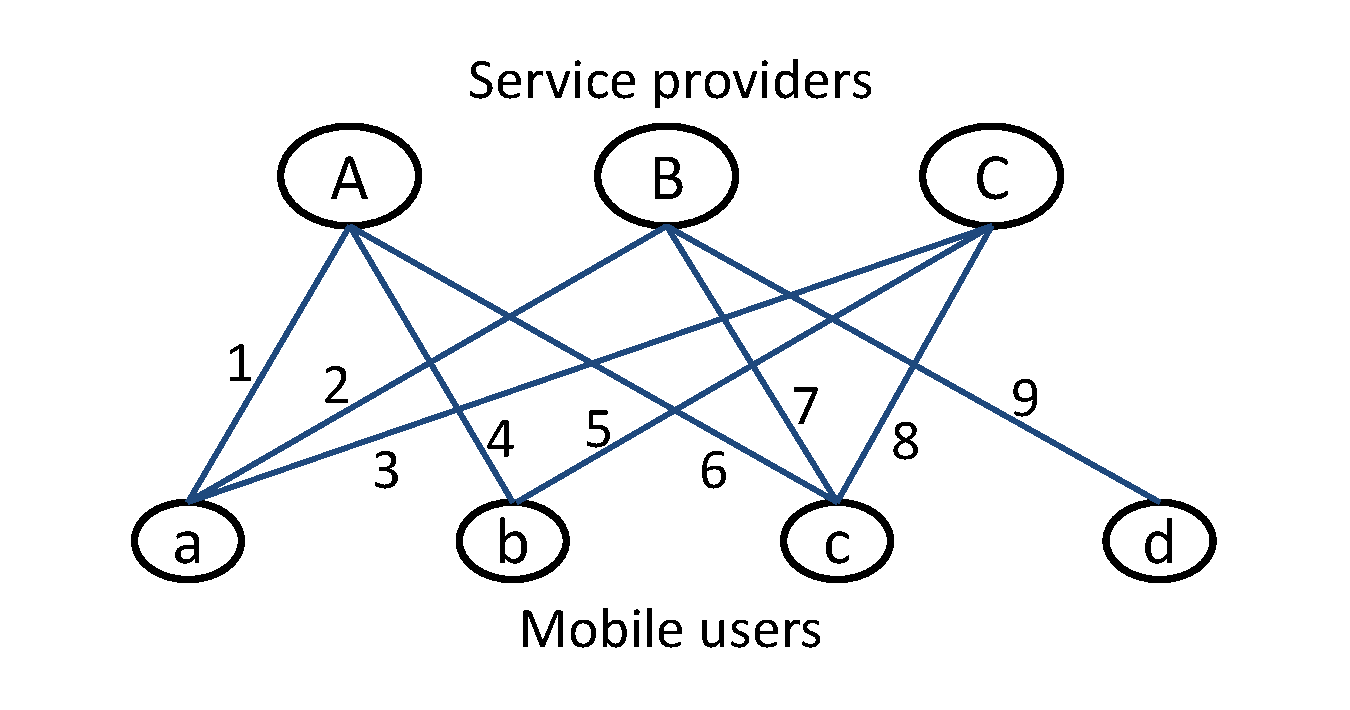
\includegraphics[scale=0.4]{./pic/layout.pdf}
%\caption{Illustration of a system with three service providers and four mobile users with nine positive usage links.}\label{fg:layout}
\caption{包含三个服务提供商和四个移动用户的系统示意图,系统中存在9条链接。}\label{fg:layout}
\end{figure}

接下来,我们通过引理\ref{lm:LCP}证明用户数据使用博弈$\ca{G}_U^{+}\triangleq(\mathcal{L}^+,\mathbb{R}_+^L,\{u_i\}_{i\in\N})$的链接需求均衡解是最佳响应函数(\ref{br1})所对应的以下线性互补问题(LCP)\cite{lcp}的解。
%In the sequel, we show that all the link demand equilibria of the usage game $\ca{G}_U^{+}\triangleq(\mathcal{L}^+,\mathbb{R}_+^L,\{u_i\}_{i\in\N})$ are the solutions to the following linear complementarity problem (LCP)\cite{lcp} formed based on the best response function (\ref{br1}), as presented in Lemma \ref{lm:LCP}. 


\begin{lm}\label{lm:LCP}

给定价格向量$\mathbf{p}^{+}$,联合数据使用量$\mathbf{x}^{+*}\in\mathbb{R}^{L^+}_+$是博弈$\ca{G}_U^{+}$的一个链接需求均衡当且仅当$\mathbf{x}^{+*}$是如下定义的线性互补性问题$LCP(W,\mathbf{x}^{+})$的解:
%Given price vector $\mathbf{p}^{+}$, a joint usage profile $\mathbf{x}^{+*}\in\mathbb{R}^{L^+}_+$ is a link demand equilibrium of game $\ca{G}_U^{+}$, if and only if $\mathbf{x}^{+*}$ is the solution to the linear complementarity problem $LCP(W,\mathbf{x}^{+})$ defined by the following inequalities:
\begin{equation}\label{eq:LCP}
%\small
\begin{cases}
    \mathbf{x}^{+}>0\\
    \mathbf{a}^{+}-\mathbf{p}^{+}-W\mathbf{x}^{+}\leq 0\\
    (\mathbf{x}^{+})^T(\mathbf{a}^{+}-\mathbf{p}^{+}-W\mathbf{x^{+}})=0
\end{cases},
\end{equation}
\noindent 其中$W$是$L^+\times L^+$维的加权邻接矩阵,其中位于$\tau(i,k)$行$\tau(i',k')$列中的元素定义为如下:
%\noindent where $W$ is a $L^+\times L^+$ weighted adjacency matrix with the element at row $\tau(i,k)$ and column $\tau(i',k')$ defined as follows:
\begin{equation}
%\small
w_{\tau(i,k),\tau(i',k')}=
\begin{cases}
  b_i+c,~~~&\mbox{if $i=i', k=k'$};\\
  b_i,~~~&\mbox{if $i=i', k\neq k'$};\\
  c-g_{ii'},~~~&\mbox{if $i\neq i', k=k'$};\\
  -g_{ii'},~~~&\mbox{if $i\neq i', k\neq k'$}.
\end{cases}
\end{equation}
\end{lm}



首先,我们声明用户数据使用博弈存在一个链接需求均衡解。
%Firstly, we claim the existence of a link demand equilibrium for the usage game.

\begin{thm}
对于用户数据使用博弈$\ca{G}_U^+$存在至少一个链接需求平衡$\mathbf{x}^{+*}$。
 % The existence of a link demand equilibrium $\mathbf{x}^{+*}$ is guaranteed for the link usage game $\ca{G}_U^+$.
\end{thm}
上述定理的证明并不复杂。由于一组链接的最佳响应定义了一个从凸紧致欧氏子空间到自身的映射,因此我们可以使用Brouwer不动点定理证明链接需求均衡的存在。 
%The proof is straightforward given the fact that the set of link best responses defines a continuous mapping from a convex compact subset of a Euclidean space into itself, based on which we can use Brouwer's fix-point Theorem to demonstrate the existence of a link demand equilibrium.


接下来,基于引理\ref{lm:LCP},我们来证明在以下条件下链路需求均衡的唯一性。
%Next, based on Lemma \ref{lm:LCP}, we show the uniqueness of the link demand equilibrium under the following conditions.


\begin{thm}\label{thm:unique}
矩阵$W$在满足对角优势条件情况下,即$\forall(i,k)\in\ca{L}$,
 % Under the diagonal dominance condition of matrix $W$, that is, $\forall (i,k)\in\ca{L}$, 
\begin{equation}\label{eq:condition}
  \begin{cases}
  %\small
  w_{(\tau(i,k),\tau(i,k))}\geq\sum_{(i',k')\in\ca{L}/(i,k)}|w_{\tau(i,k),\tau(i',k')}|, \\
  w_{(\tau(i,k),\tau(i,k))}\geq\sum_{(i',k')\in\ca{L}/(i,k)}|w_{\tau(i',k'),\tau(i,k)}|,
  \end{cases}
 \end{equation}
 用户数据使用博弈$\ca{G}_U^+$存在以下唯一的链接需求均衡,
% the link usage game $\ca{G}_U^+$ admits a unique link demand equilibrium, given by
  \begin{equation}\label{eq:LDE}
  	\mathbf{x}^{+*}=W^{-1}(\mathbf{a}^{+}-\mathbf{p}^{+}).
  \end{equation}
\end{thm}
\begin{proof}
为了证明链接需求均衡的唯一性,我们证明用户数据使用博弈$\ca{G}_U^+$在满足条件(\ref{eq:condition})的情况下属于凹博弈。收益函数$\mathbf{u}^+(\mathbf{x})$ 的雅克比矩阵$\nabla\mathbf{u}^+(\mathbf{x})$ 如下所示, 
\begin{equation}
\begin{array}
[c]{lll}%
\mathbf{X}&=
  \begin{bmatrix}
   \frac{\partial^2u_1^+(\mathbf{x}^+)}{{\partial x^{+}_1}^2}  &  \frac{\partial^2u_1^+(\mathbf{x}^+)}{\partial x^{+}_1\partial x^{+}_2}  &  ~\cdots  &  \frac{\partial^2u_1^+(\mathbf{x}^+)}{\partial x^{+}_1\partial x^{+}_{L^+}}\\
   \frac{\partial^2u_2^+(\mathbf{x}^+)}{\partial x^{+}_2\partial x^{+}_1}  &  \frac{\partial^2u_1^+(\mathbf{x}^+)}{{\partial x^{+}_2}^2}  &  ~\cdots  &  \frac{\partial^2u_2^+(\mathbf{x}^+)}{\partial x^{+}_2\partial x^{+}_{L^+}}\\
    \vdots  &  \vdots  &  ~\ddots  &  \vdots\\
   \frac{\partial^2u_{L^+}^+(\mathbf{x}^+)}{\partial x^{+}_{L^+}\partial x^{+}_1}  &  \frac{\partial^2u_{L^+}^+(\mathbf{x}^+)}{\partial x^{+}_{L^+}\partial x^{+}_2}  &  ~\cdots  &  \frac{\partial^2u_{L^+}^+(\mathbf{x}^+)}{{\partial x^{+}_{L^+}}^2}\\
  \end{bmatrix}\\[45pt]  
  &=-W
\end{array}
\end{equation}
在条件(\ref{eq:condition})的情况下,矩阵$W$即满足行对角占优同时也满足列对角占优,同时其转置$W^T$也是对角占优的。于是我们有
\begin{equation}
 \nabla\mathbf{u}^+(\mathbf{x}) + \nabla\mathbf{u}^+(\mathbf{x})^T = -W - W^T
\end{equation}
是严格对角占优且对称的。根据文献\cite{Horn85}中的现有结论,当一个严格对角占优对称矩阵的对角元素为非负实数时,该矩阵为正定的。因此在这里,我们有$\nabla\mathbf{u}^+(\mathbf{x}) + \nabla\mathbf{u}^+(\mathbf{x})^T$是负正定的矩阵。依据文献\cite{econometrica}中的定理,我们可以得到$\nabla\mathbf{u}^+(\mathbf{x})$是严格对角凹的。因此,利用文献\cite{econometrica}中定理2的结果,我们可以得到博弈$\ca{G}_U^+$ 存在唯一的链接需求均衡。
\end{proof}
定理\ref{thm:unique}的证明基于以下事实:在条件\ref{eq:condition}下,式(\ref{eq:LCP})所定义的线性互补问题$LCP(W,\mathbf{x}^{+})$对应于一个凹博弈(Concave game),因此解$\mathbf{x}^{+*}$是唯一的。基于引理\ref{lm:LCP}所述的,即问题$LCP(W,\mathbf{x}^{+})$的解与博弈$\ca{G}_U^{+}$的均衡点对应,我们可据此确定链接需求均衡点在特定条件下的唯一性。详细的证据参见附录A。正如(9)所示,我们可以显式地将链接需求均衡点表述为$\mathbf{a}^{+}$和$\mathbf{p}^{+}$的线性组合。因此,当达到链接需求均衡点时每名用户$i\in\N$的使用消耗量$\sum_{k\in\K}x^{+*}_{\tau(i,k)}$应是$\mathbf{a}=(a_1,\cdots,a_N)$和$\mathbf{p}=(p_1,\cdots,p_K)$的线性函数。

%The proof of Theorem \ref{thm:unique} follows from the fact that under the condition (\ref{eq:condition}), the linear complementarity problem $LCP(W,\mathbf{x}^{+})$ defined in (\ref{eq:LCP}) corresponds to a concave game, thus has a unique solution $\mathbf{x}^{+*}$. Since the solution of problem $LCP(W,\mathbf{x}^{+})$ corresponds to the equilibrium of the game $\ca{G}_U^{+}$ as indicated by Lemma \ref{lm:LCP}, we can thereby establish the conditional uniqueness of the link demand equilibrium. The detailed proof has been relegated to the Appendix A. As shown in (\ref{eq:LDE}), we can explicitly express the link usage equilibrium as a linear combination of $\mathbf{a}^{+}$ and $\mathbf{p}^{+}$. As a result, the usage consumption of each user $i\in\N$ under the link demand equilibrium, $\sum_{k\in\K}x^{+*}_{\tau(i,k)}$, should be a linear function of $\mathbf{a}=(a_1,\cdots,a_N)$ and $\mathbf{p}=(p_1,\cdots,p_K)$. 

\section{理性服务提供商之间的定价博弈}\label{sec:stageI}
%\section{Pricing Game among Rational Service Providers}\label{sec:stageI}
在上一节中,我们已经说明了阶段\uppercase\expandafter{\romannumeral2}数据使用博弈存在链接需求均衡点并且均衡点具有唯一性。接下来,我们来说明第一阶段无线提供商服务价格的确定。从理论上讲,每个服务提供商都可以在一个连续的价格变量上优化其收入。实际上,服务提供商宣布的价格通常落在离散样本空间内,并在一组离散价格水平上服从指定概率分布。为了刻画这个特征,在我们所关注的定价博弈中,服务提供商针对其他用户的策略通过选择概率定价策略来最大化其期望收入。在本节中,我们考虑传统的情况,即理性的服务提供商客观地评估自己的收入和其他用户的策略。我们确定了博弈混合策略定价均衡点的存在性。
%In the previous section, we have shown the existence and uniqueness of the link demand equilibrium for the usage game in Stage II. Next, we move on to the determination of service prices for wireless providers in Stage I. Theoretically, each service provider can optimize his revenue over a continuous price variable. While in practice, the price announced by the service provider usually falls within a discrete sample space with a probabilistic distribution specified over a set of discrete price levels. To capture this feature, our discussion focuses on the pricing game that service providers maximize their expected revenues via choosing probabilistic pricing strategies against other users' strategies. In this section, we consider the conventional scenario where rational service providers evaluate their own revenue and other users' strategies objectively. We establish the existence of a mixed-strategy pricing equilibrium for the game. 

\subsection{混合策略定价均衡点的存在性}\label{sec:exist1}
我们将提供商$k$的混合策略定义为$\pi_{k}=(\pi_k(p_{k}^1),\pi_k(p_{k}^2),\cdots,\pi_k(p_{k}^{M_{k}}))\in\Delta \mathcal{P}_{k}$, 其中$\pi_k(p_{k}^m)\in[0,1]$是提供者$k$选择价格$p_{k}^m\in\mathcal{P}_k$的概率。既而我们有$\sum_{m=1}^{M_k}\pi_k\left(p_{k}^{m}\right)=1$。我们定义一个联合的混合策略定价策略$\pi=(\pi_{1},\cdots,\pi_{K})$为一个笛卡尔积$\Delta \mathcal{P}\triangleq\prod_{k\in\K} \Delta \mathcal{P}_{k}$。遵循冯·诺依曼·摩根斯坦恩的期望效用理论(EUT)\cite{Von},在混合策略下,提供商$k\in\K$的收入$z_k^{EUT}$可以表示为
%We define the mixed-strategy of provider $k$ as $\pi_{k}=(\pi_k(p_{k}^1),\pi_k(p_{k}^2),\cdots,\pi_k(p_{k}^{M_{k}}))\in\Delta \mathcal{P}_{k}$, where $\pi_k(p_{k}^m)\in[0,1]$ is the probability that provider $k$ chooses price $p_{k}^m\in\mathcal{P}_k$, with $\sum_{m=1}^{M_k}\pi_k\left(p_{k}^{m}\right)=1$. A joint mixed-strategy pricing profile $\pi=(\pi_{1},\cdots,\pi_{K})$ is defined as a joint probability distribution over the Cartesian product $\Delta \mathcal{P}\triangleq\prod_{k\in\K} \Delta \mathcal{P}_{k}$. Following Von Neumann-Morgenstern's Expected Utility Theory (EUT) \cite{Von}, the revenue of a provider $k\in\K$ under mixed strategies, denoted by $z_k^{EUT}$, can be written as
\begin{equation}\label{eq:EUT}
%\small
z_{k}^{EUT}(\pi_{k},\pi_{-k})=\sum_{\mathbf{p}\in \mathcal{P}}\left(\prod_{k\in\K}\pi_k(p_{k})\right)v_k,
\end{equation}
其中$\pi_{-k}\in\prod_{k'\in\K,k'\neq k}\Delta\mathcal{P}_{k'}$表示除提供商$k$外的所有其他提供商的混合策略。这里,$v_k$可以根据(\ref{eq:SPrev})计算得到,其中总数据使用量从阶段\uppercase\expandafter{\romannumeral2}的链路需求均衡$\mathbf{x}^{+*}$获得(如上节\ref{sec:stageII}所述)。
%where $\pi_{-k}\in\prod_{k'\in\K,k'\neq k}\Delta\mathcal{P}_{k'}$ denotes the mixed strategies of all other providers except provider $k$. Here, $v_k$ can be calculated according to (\ref{eq:SPrev}), in which the aggregated consumption is obtained from the link demand equilibrium $\mathbf{x}^{+*}$ of Stage I (as discussed in Section \ref{sec:stageII}).

我们根据期望效用理论将定价博弈重新定义为$\mathcal{G}_P^{EUT}\triangleq(\mathcal{K},\Delta\mathcal{P},\{z^{EUT}_k\}_{k\in\mathcal{K}})$。定价博弈的混合策略纳什均衡定义如下。
%We redefine the pricing game under Expected Utility Theory as $\mathcal{G}_P^{EUT}\triangleq(\mathcal{K},\Delta\mathcal{P},\{z^{EUT}_k\}_{k\in\mathcal{K}})$. The mixed-strategy Nash equilibrium for the pricing game is defined as follows.

\begin{df}[混合价格策略均衡]
我们认为如果对于每个服务提供商$k\in\mathcal{K}$,以下条件满足
%The mixed-strategy pricing profile $\pi^*=(\pi_{1}^*,\cdots,\pi_{K}^*)\in\Delta\mathcal{P}$ is a mixed-strategy pricing equilibrium, if for every service provider $k\in\mathcal{K}$, we have
\begin{equation}\label{eq:exrev1}
z_{k}(\pi_{k}^*,\pi_{-k}^*)\ge z_{k}(\pi_{k},\pi_{-k}^*),~\forall \pi_k\ne\pi_k^*.
\end{equation}
则混合定价策略$\pi^*=(\pi_{1}^*,\cdots,\pi_{K}^*)\in\Delta\mathcal{P}$是一个混合策略价格均衡。
\end{df}

在下面的定理中,我们说明了博弈$\mathcal{G}^{EUT}_{P}$中存在混合策略定价均衡。
%In the following Theorem, we show the existence of a mixed-strategy pricing equilibrium for the game $\mathcal{G}^{EUT}_{P}$.
\begin{thm}\label{thm:exist}
定价博弈$\mathcal{G}^{EUT}_{P}$至少存在一个混合策略的定价均衡$\pi^{*}\in\Delta\mathcal{P}$。
%There exists at least one mixed-strategy pricing equilibrium $\pi^{*}\in\Delta\mathcal{P}$ for the pricing game $\mathcal{G}^{EUT}_{P}$.
\end{thm}
\begin{proof}
根据我们的模型,每个无线服务提供商$k\in\K$会从$M_k$个价格中选择并进行定价。由于服务提供商的数量和每个服务提供商的定价策略空间都是有限的,因此定价游戏$\mathcal{G}^{EUT}_{P}$属于有限博弈。而混合策略定价均衡$\pi^*$是最佳响应对应(Best response correspondence)的固定点。根据Kakutani不动点定理,价格博弈$\mathcal{G}^{EUT}_{P}$至少存在一个混合策略的纳什均衡\cite{osborne}。
%According to our model, each wireless service providers $k\in\K$ sets the price from $M_k$ pricing strategies. Since both the number of service providers and the pricing strategy space of each service provider are finite, the pricing game $\mathcal{G}^{EUT}_{P}$ falls into the class of finite game. A mixed-strategy pricing equilibrium $\pi^*$ is a fixed point of the best-response correspondence. By the Kakutani's fixed point theorem, the existence of at least one mixed-strategy Nash equilibrium is guaranteed for the pricing game $\mathcal{G}^{EUT}_{P}$\cite{osborne}.
\end{proof}

在实际中,为了避免收敛时间慢和寻找平衡点所需的不必要开销,我们可以考虑落在混合策略纳什平衡点附近足够小邻域内的近似平衡点。我们因此定义以下$\epsilon$价格均衡:
%In practice, to avoid slow convergence time and unnecessary overhead of finding equilibria, we can consider approximate equilibrium solutions that fall within a small enough neighborhood of the mixed-strategy Nash Equilibrium. Consider an $\epsilon$-pricing equilibrium defined as follows:
\begin{df}[$\epsilon$-价格均衡]
如果对于每个服务提供商$k\in\mathcal{K}$,我们有
%A mixed-strategy pricing profile $\pi^*=(\pi_{1}^*,\cdots,\pi_{K}^*)\in\Delta\mathcal{P}$ is an $\epsilon$-pricing equilibrium, if for each service provider $k\in\mathcal{K}$, we have
\begin{equation}\label{approxNE}
%\small
z_{k}(\pi_{k}^*,\pi_{-k}^*)\ge z_{k}(\pi_{k},\pi_{-k}^*) + \epsilon,~\forall \pi_k\ne\pi_k^*.
\end{equation}
则混合策略定价均衡$\pi^*=(\pi_{1}^*,\cdots,\pi_{K}^*)\in\Delta\mathcal{P}$是一个$\epsilon$定价均衡。
\end{df}
由定理\ref{thm:exist},我们可以直接得出$\epsilon$定价平衡的存在性。为了明确地寻找一个$\epsilon$定价均衡,我们可以诉诸于论文\cite{MYCISS16}中第五节中提出的集中式算法。
%The existence of an $\epsilon$-Pricing Equilibrium follows directly from Theorem \ref{thm:exist}. To explicitly search for an $\epsilon$-pricing equilibrium, we can resort to a centralized algorithm proposed in Section V of our previous paper \cite{MYCISS16}.

%\section{Pricing Game among Service Providers with Bounded Rationality}\label{sec:stageI2}
\section{有限理性服务提供商之间的定价博弈}\label{sec:stageI2}
在第五节中,服务提供商的收入是基于期望效用理论建模的,其前提假设是完全理性的提供商在价格竞争中采取客观的行为。但是我们观察到,卖方在实践中的行为通常偏离经典的期望效用理论\cite{Kahneman}所预测的理性行为路径。具体来说,服务提供商可能会对其对手的概率定价策略以及自己的收益函数进行主观评估。我们使用展望理论(PT)来捕捉定价博弈中的行为因素。
%In Section V, service provider's revenue is modeled based on Expected Utility Theory assuming fully rational providers acting objectively during the pricing competition. However, it has been observed that, sellers' behavior in practice usually deviate from the rational path predicted by this classic Expected Utility Theory \cite{Kahneman}. Specifically, service providers may have subjective evaluation on the probabilistic pricing strategy of their opponents as well as their own revenue functions, which are used for decision making. In order to capture such behavioral factors in our proposed pricing game, we resort to Prospect Theory (PT).

\subsection{展望理论下的提供商收入期望}
%\subsection{Provider's Expected Revenue under Prospect Theory}

我们考虑展望理论的两个主要特征。第一个是\emph{概率失真效应},指现实中决策者倾向于看重小概率事件,但是看轻中等和大概率事件。
%具体而言,这种特性可以通过将客观概率$p$映射到主观概率的概率失真函数$w(p)$来刻画。
我们考虑同类服务提供商并使用较为广泛的概率失真函数有Prelec函数\cite{Prelec}。则
%We consider two main features of Prospect Theory. The first one is the \emph{probability distortion effect}, which states that decision maker is prone to overweigh events with small probability, but underweight medium and large probability events. Specifically, this characteristic can be captured by a probability distortion function $w(p)$ that maps an objective probability $p$ to a subjective one. A widely used probability distortion function is the Prelec function \cite{Prelec}:
%\begin{equation}\label{eq:distortion}
%w(p)=\exp(-(-\ln p)^{\alpha}), 0<\alpha\leq 1,
%\end{equation}
%其中$p$是事件的真实概率,$\alpha$是概率失真参数,$w(p)$是对应的主观概率。图\ref{fg:dist_func}阐明了具有不同参数的概率失真函数(\ref{eq:distortion})。我们可以看到所有曲线在点$1/e$相交。此外,当$0\leq p < 1/e$时,函数是凸的,$w(p)<p$(即低估客观概率);而当$1/e\leq p<1$时,函数是凹的,我们有$w(p)\geq p$(即高估客观规律)。失真参数$\alpha$的值越小,则概率失真效应越明显。当$\alpha$设置为1时,该函数即变为客观概率。
提供商的主观评估可以通过式(\ref{eq:distortion})中给出的具有相同$\alpha$取值的失真函数来表征。同时,我们假设服务提供商能够客观地评估自身的策略。因而在展望理论下,用户$k$对联合定价策略$\mathbf{p}\in\Delta\mathcal{P}$的评估可以表示为$\pi_k(p_k)w(\prod_{k'\in\K,k'\neq k}\pi_{k'}(p_{k'}))$。
%where $p$ is the real probability of an event, $\alpha$ is the probability distortion parameter, and $w(p)$ is the corresponding subjective probability. Fig. \ref{fg:dist_func} illustrates the probability distortion function (\ref{eq:distortion}) with different parameters. We can see that all the curves intersect at the point $1/e$. Besides, we have when $0\leq p < 1/e$, the function is convex, and $w(p)<p$ (under-weighting); when $1/e\leq p<1$, the function is concave, and we have $w(p)\geq p$ (over-weighting). A smaller value of distortion parameter $\alpha$ corresponds to a more significant probability distortion effect. When $\alpha$ is set to 1, the function reduces to the objective probability. In our work, we consider homogeneous service providers whose subjective evaluation can be characterized by the distortion function given in (\ref{eq:distortion}) with a same fixed value of $\alpha$. Meanwhile, we assume that service providers are able to evaluate their own strategies objectively. Thus, user $k$'s evaluation for a joint pricing strategy $\mathbf{p}\in\Delta\mathcal{P}$ under Prospect Theory can be expressed as $\pi_k(p_k)w(\prod_{k'\in\K,k'\neq k}\pi_{k'}(p_{k'}))$.
%\begin{figure}
%\centering
%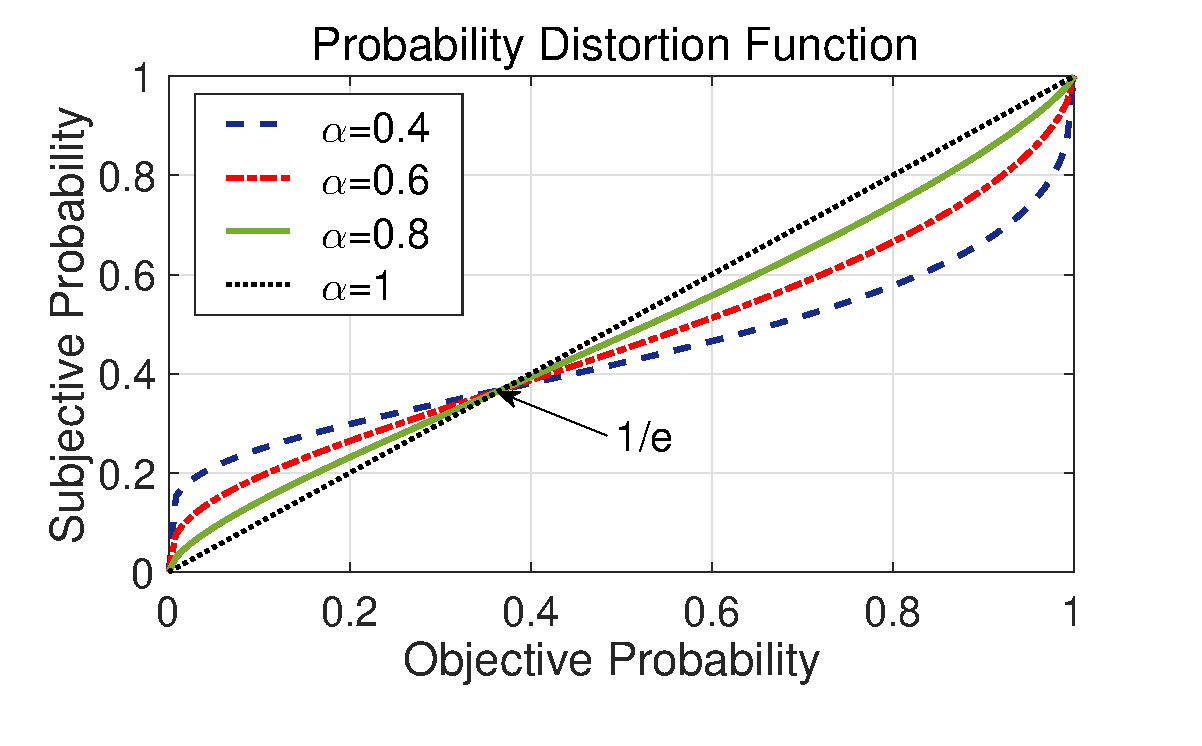
\includegraphics[scale=0.58]{./pic/dist_func.eps}
%%\caption{Probability distortion functions under different distortion parameters $\alpha$.}\label{fg:dist_func}
%\caption{失真参数$\alpha$不同取值下的概率失真函数。}\label{fg:dist_func}
%\vspace{0.1cm}
%\centering
%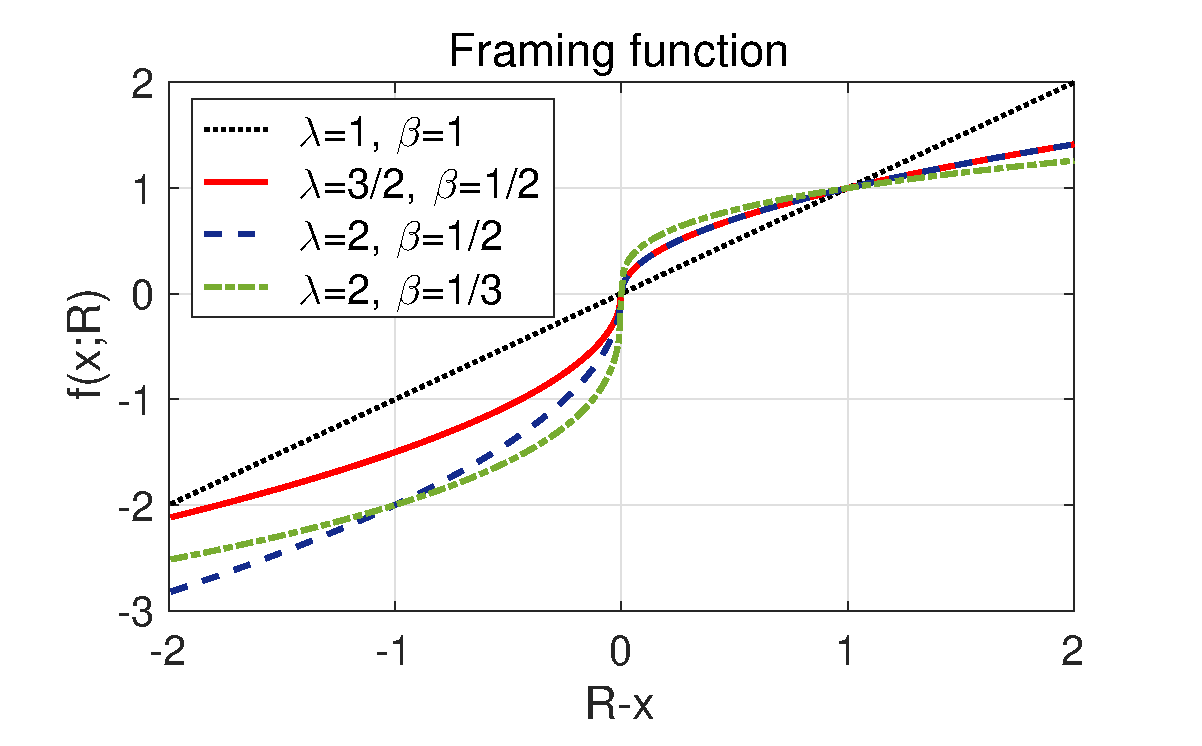
\includegraphics[scale=0.58]{./pic/fram_func.eps}
%%\caption{Framing functions under different utility aversion parameters $\beta$ and loss penalty parameter $\lambda$.}\label{fg:fram_func}
%\caption{不同效用规避参数$\beta$和损失惩罚参数$\lambda$下的框架函数。}\label{fg:fram_func}
%\end{figure}

我们考虑的展望理论的另一个特征是\emph{效用框架效应}。此效应反映了每个服务提供商对自己的收益进行主观评估的实际情况。
%实际中,仅当其收入超过参照点$R$($R$无需等于零)时,每名用户才会将其视为收益增益,否则将视为收益损失。同样,在给定参考点$R$的情况下,S型单调框架函数$f(\cdot)$会进一步调整客观收入,其中函数在$v>R$侧为凹函数,而在$v<R$一侧是凸函数。此外,在$R$附近,收益损失比收益增益增长得更快,表明收益损失的边际效用大于收益增益的边际效用。
在本文中,我们使用基于Kahneman提出的框架函数\cite{Kahneman},
%Another characteristic of Prospect Theory we considered is the \emph{utility framing effect}. This effect captures the practical situation where each service provider has subjective evaluation of her own payoff. In practice, each user might consider her payoff as a gain only if it is above a reference point $R$ (not necessarily equals zero), and consider it as a loss otherwise. Also, given the reference point $R$, the objective payoff is further tuned by a S-shaped monotone framing function $f(\cdot)$, which is concave at the side where $v>R$, and convex at the side where $v<R$. In addition, in the neighborhood of $R$, the losses loom larger than gains indicating that the marginal utility in losses is larger than in gains. In this work, we use a framing function based on the one proposed in \cite{Kahneman},
%\begin{equation}\label{eq:framing}
%f(x;R)=
%\begin{cases}
%(v - R)^{\beta}, &v\geq R\\
%-\lambda(R-v)^{\beta}, &v<R
%\end{cases}
%\end{equation}
%其中参数$0<\beta\leq 1$和$\lambda\geq 1$分别用于刻画风险规避和损失规避的因素。图\ref{fg:fram_func}展示了不同参数取值下的框架函数。特别地,当博弈参与者收入远离参照点时,$\beta$值越大,表示风险规避程度较小;$\lambda$值的增大则刻画了博弈参与者在客观上经历等同的收益的损失和增益时,所主观上体验到的损失要大于所体验到的增益。容易看出,当$\beta=\lambda=1$时,主观收益曲线与原始的客观收益曲线一致。我们假设每个服务提供商$k$基于式(\ref{eq:framing})来评估其收入。
则在展望理论模型下,服务提供商$ k\in\K$的预期收入$z_k^{PT}$可写为
%where the parameters $0<\beta\leq 1$ and $\lambda\geq 1$ model the risk aversion and loss aversion respectively. Fig. \ref{fg:fram_func} illustrates the framing function with different parameters. In particular, a larger $\beta$ characterizes less degree of risk aversion when the player's payoff is away from the reference point; and a larger $\lambda$ captures the greater loss experienced by the player with her payoff being reduced by a certain amount, in comparison to the corresponding gain she experiences with the same amount of the payoff increase. It is easy to see that when $\beta=\lambda=1$, the subjective payoff boil down to the original objective payoff. We assume each service provider $k$ evaluate her revenue using (\ref{eq:framing}) with parameter $\beta_k$, and reference point $R_k, \forall k\in\K$. Under Prospect Theory model, the expected revenue $z_k^{PT}$ of service provider $k\in\K$ can be written as

\begin{equation}\label{eq:PT}
%\small
z_{k}^{PT}(\pi_{k},\pi_{-k})=\sum_{\mathbf{p}\in \mathcal{P}}\pi_k(p_k)w\left(\prod_{k'\in\K,k'\neq k}\pi_{k'}(p_{k'})\right)f_k(v_k).
\end{equation}

我们将展望理论讨论下的定价博弈表示为$\mathcal{G}_P^{PT}\left(\mathcal{K},\Delta\mathcal{P},\{z_k^{PT}(R_k)\}_{k\in\mathcal{K}}\right)$,并在下一节中重新讨论价格博弈的均衡解的存在。
%We denote the pricing game under Prospect Theory as $\mathcal{G}_P^{PT}\left(\mathcal{K},\Delta\mathcal{P},\{z_k^{PT}(R_k)\}_{k\in\mathcal{K}}\right)$, and revisit the existence of equilibrium solution for the pricing game in the next section.


\subsection{混合策略定价均衡点的存在性}
在节\ref{sec:exist1}中建立混合策略纳什均衡的存在时,概率上期望收入(\ref{eq:EUT})的线性性起着关键作用。然而正如前一节所述,在展望理论中参与者对通过非线性失真函数建模的信念进行主观加权。因此,我们需要重新评估游戏定价均衡的存在。我们首先对展望理论下的混合策略纳什均衡给出以下定义。
%The mixed-strategy Nash equilibrium requires players optimally choosing their strategies given their beliefs of other players' strategies. The linearity of expected revenue (\ref{eq:EUT}) in probabilities plays a key role in establishing the existence of a mixed-strategy Nash equilibrium. However, as mentioned in the previous section, players will subjectively weight their beliefs modeled via non-linear distortion function on the probabilities under Prospect Theory. Thus, we need to reevaluate the existence of the pricing equilibrium of the game. We first provide the following definition for the mixed-strategy Nash equilibrium under Prospect Theory.

\begin{df}[展望理论(PT)下的混合策略价格均衡]
如果对于每个服务提供商$k\in\mathcal{K}$有,
%We call a mixed-strategy profile $\pi^*=(\pi_{1}^*,\cdots,\pi_{K}^*)\in\Delta\mathcal{P}$ a mixed-strategy pricing equilibrium under Prospect Theory, if for each service provider $k\in\mathcal{K}$,
\begin{equation}
%\small
z_{k}^{PT}(\pi_{k}^*,\pi_{-k}^*)\geq z_{k}^{PT}(\pi_{k},\pi_{-k}^*),~\forall \pi_k\ne\pi_k^*.
\end{equation}
则我们称该混合价格策略$\pi^*=(\pi_{1}^*,\cdots,\pi_{K}^*)\in\Delta\mathcal{P}$为展望理论下的混合策略定价均衡。
\end{df}

我们在以下定理中证明,当每个服务提供商的参考点固定时,我们的定价博弈$\mathcal{G}_{P}^{PT}$存在混合纳什均衡。
%We show in the following Theorem that our pricing game $\mathcal{G}_{P}^{PT}$ admits a mixed Nash equilibrium under the condition that each service provider's reference point is fixed.
\begin{thm}\label{thm:exist2}
如果服务提供商的参考点$\{R_k\}_{k\in\mathcal{K}}$都是固定的,则定价博弈$\mathcal{G}^{PT}_{P}$存在至少一个混合策略均衡点$\pi^{*}\in\Delta\mathcal{P}$。
%At least one mixed-strategy pricing equilibrium $\pi^{*}\in\Delta\mathcal{P}$ is guaranteed for the pricing game $\mathcal{G}^{PT}_{P}$, if service providers' reference points $\{R_k\}_{k\in\mathcal{K}}$ are all fixed.
\end{thm}
\begin{proof}
对于每个$k\in\mathcal{K}$,给定任意$R_k\in \mathbb{R}$和$\pi_{-k}\in\Delta\mathcal{P}_{-k}$,对于每个价格$p_k\in\mathcal{P}_k$,期望收入$z_{k}^{PT}(\pi_k, \pi_{-k})$是$\pi_k(p_k)$的线性函数。由于$\Delta\mathcal{P}_{k}$是紧凑集合,因此最佳响应策略集$\bold{B}_k(\pi_{-k})\triangleq\{\pi'_k\in\Delta\mathcal{P}:z_{k}^{PT}(\pi'_k, \pi_{-k})\geq z_{k}^{PT}(\pi_k, \pi_{-k})\}$是非空的,紧凑的且凸的。注意到$\pi_{-k}$是通过$w(\cdot)$以$\pi_{-k}(p_{-k})=\prod_{k'\in\K, k'\neq k}\pi_{k'}(p_{k'})$的形式引入到$z_{k}^{PT}(\cdot)$ 。由于式(\ref{eq:distortion})中给出的概率失真函数$w(p)$是$p$的连续函数,因此$z_{k}^{PT}(\pi_k, \pi_{-k})$对于每个$\pi_{-k}\in\Delta\mathcal{P}_{-k}$是连续的。根据Berge最大值定理,最佳响应对应$B_k(\pi_{-k})$是上半连续的。根据Kakutani固定点定理,存在$\pi^*\in\Delta\mathcal{P}$,使得对于所有$k\in\mathcal{K}$,$\pi_k\in B_k(\pi_{-k})$成立。因此,定理\ref{thm:exist2}中的论述成立。
%For each $k\in\mathcal{K}$, given any $R_k\in \mathbb{R}$ and $\pi_{-k}\in\Delta\mathcal{P}_{-k}$, the expected revenue $z_{k}^{PT}(\pi_k, \pi_{-k})$ is linear in $\pi_k(p_k)$ for each $p_k\in\mathcal{P}_k$. As $\Delta\mathcal{P}_{k}$ is compact, the set of best responses strategies: $\bold{B}_k(\pi_{-k})\triangleq\{\pi'_k\in\Delta\mathcal{P}:z_{k}^{PT}(\pi'_k, \pi_{-k})\geq z_{k}^{PT}(\pi_k, \pi_{-k})\}$ is nonempty, compact and convex valued. Note that $\pi_{-k}$ enters $z_{k}^{PT}(\cdot)$ via $w(\cdot)$ in the form of $\pi_{-k}(p_{-k})=\prod_{k'\in\K, k'\neq k}\pi_{k'}(p_{k'})$. Since the probability distortion function $w(p)$ given in (\ref{eq:distortion}) is continuous in $p$, $z_{k}^{PT}(\pi_k, \pi_{-k})$ is continuous in $\pi_{-k}$ for each $\pi_{-k}\in\Delta\mathcal{P}_{-k}$. By Berge's Maximum Theorem, the correspondence $B_k(\pi_{-k})$ is upper hemicontinuous. And by Kakutani's Fixed Point Theorem, there exists some $\pi^*\in\Delta\mathcal{P}$ such that $\pi_k\in B_k(\pi_{-k})$ for all $k\in\mathcal{K}$. Therefore, the claim in the Theorem \ref{thm:exist2} holds.
\end{proof}


\noindent\textbf{备注:}我们关于展望理论混合策略定价均衡点是否存在的讨论针对较为普遍的情况,即服务提供商收益参考点为固定值,且由服务商自行确定。然而当参照点不固定时,很容易发现,即使在仅有两个博弈玩家且每人只有两个纯策略的情况下,混合策略定价均衡点也不一定存在。而如果服务提供商$k$参照点的取值同时取决于其他人的参照点,则均衡点的分析会变得更为复杂。
%\noindent\textbf{Remarks.} Our discussion about the existence of mixed-strategy pricing equilirbium under Prospect Theory is for fairly common case where service providers' reference points $\{R_k\}_{k\in\K}$ are fixed and determined solely by service providers themselves. Nevertheless, when the reference points are not fixed, it can be easily shown that the mixed-strategy pricing equilibrium might not exist even for a two-player case, where each player has two pure pricing strategy. If the reference point of service provider $k$ is also dependent on others, the equilibrium analysis will become even complicated.

\subsection{混合策略定价均衡的分布式学习算法}
%\subsection{Distributed Learning Algorithm for Finding Mixed-strategy Pricing Equilibrium}
在本节中,我们为有限理性的服务提供商设计寻找混合策略定价均衡的算法,而其中的挑战主要来自展望理论模型的效用框架效应。具体来说,参数$\beta_k$和$R_k$都是仅服务提供商$k$自己所掌握的私有信息。因而没有一个集中式的个体知道所有服务提供商的效用函数,而这恰恰是对于计算$\epsilon$-混合策略纳什均衡所需的。
%In this section, we develop the algorithm for service providers of bounded rationality to find a mixed-strategy pricing equilibrium. One main challenge is raised by the utility framing effect of Prospect Theory model. Specifically, the parameters $\beta_k$ and $R_k$ are all private information only known to service provider $k\in\K$. As a result, no centralized party has the knowledge of all service providers' utility function, which are necessary for calculating an $\epsilon$-mixed-strategy Nash equilibrium. 

为了应对这一挑战,我们采用了基于虚拟对弈的分布式学习算法。通过该算法,博弈参与者可以通过观察对手的动作学习得到均衡策略。基于纳什均衡和最佳响应之间的直接联系,如果在算法结束时信念成功收敛,则可以达到纳什均衡。但是,这种标准的虚拟对弈算法并不总是能很好地发挥作用,因为在某些博弈中这些信念无法收敛。在某些其他情况中,虽然信念收敛,但是混合策略或收入无法收敛。
%To tackle this challenge, we resort to distributed Fictitious Play based learning algorithm, through which players can learn to play out the equilibrium strategies via observations of their opponents' actions. Given the direct connection between the Nash equilibrium and the best response, it is expected that a Nash equilibrium should be obtained if the beliefs converge successfully at the end of the algorithm. However, such kind of standard Fictitious Play algorithm does not always work well: the beliefs can not converge for some games;
%\footnote{A sufficient condition for convergence is that the game belongs to potential game, and a sufficient condition for non-convergence of beliefs is the existence of cycles in the game.}
在其他一些情况下,尽管信念会聚,但混合策略或收益不会收敛。在一些标准虚拟对弈中策略和收益不收敛的原因是由于博弈策略不是信念的连续函数。因此,我们采用了随机虚拟对弈算法(标准虚拟对弈的一个修改版本);其中,每个博弈参与者所做出的策略都是平滑的最佳响应,而不是标准的最佳响应。
%in some other cases, although the beliefs converge, the mixed-strategy or the payoff does not converge. The non-convergence of strategies and payoffs in standard Fictitious Play is due to the fact that played strategy is not a continuous function of beliefs. Therefore, we employ the Stochastic Fictitious Play algorithm, a modified version of Fictitious Play, in which each player makes smooth best response instead of the standard best response.

\begin{df}[平滑最佳响应]
对于收益为$z^{PT}_k(\pi_k,\pi_{-k})$的博弈参与者$k\in\mathcal{K}$,给定其对手的联合混合策略$\p_{-k}$,平滑最佳响应$\bold{b}_k(\p_{-k};\eta)\in\Delta\mathcal{P}_k$对应于以下定义的混合策略:
%For each player $k\in \mathcal{K}$ with payoff $z^{PT}_k(\pi_k,\pi_{-k})$, given its opponents' joint mixed-strategy $\p_{-k}$, the smooth best response $\bold{b}_k(\p_{-k};\eta)\in\Delta\mathcal{P}_k$ corresponds to the mixed-strategy defined as:
\begin{equation}\label{sbr0}
\bold{b}_k(\p_{-k};\eta)=\underset{\pi_k\in\Delta\mathcal{P}_k}{\arg\max}\left\{z_k^{PT}(\pi_k,\p_{-k})+\frac{1}{\eta}E(\pi_k)\right\},
%=&\underset{\pi_n\in\Delta\mathcal{A}_n}{\arg\max}\left\{\sum_{i=1}^{|\mathcal{A}_n|}q(a_{n,i})R_n(a_{n,i},\p_{-n})+\frac{1}{\beta}\upsilon_n(\pi_n)\right\}.
\end{equation}
其中$\eta>0$是温度参数,$E(\pi_k):\Delta\mathcal{P}_k\rightarrow \mathbb{R}$是严格可微的凹函数,导致当$\pi_k$趋近于$\Delta\mathcal{P}_k$的边界时,$E(\pi_k)$具有无限大的斜率。
%where $\eta>0$ is a temperature parameter and $E(\pi_k):\Delta\mathcal{P}_k\rightarrow \mathbb{R}$ is a strictly differentiable and concave function, causing an infinite slope of $E(\pi_k)$ as $\pi_k$ approaches the boundary of $\Delta\mathcal{P}_k$.
\end{df}

由于平滑最佳响应在$\pi_{-k}$中是连续的,因此信念的收敛意味着混合策略的收敛。我们采用常用的熵形式的平滑函数$E(\pi_k)=-\sum_{m=1}^{M_k}\pi_k(p_{k}^{m})\ln \pi_k(p_{k}^{m})$。这种情况下当$\eta\rightarrow\infty$时,平滑最佳响应$\bold{b}_k(\pi_{-k}; \eta)$恰好可化为标准的最佳响应。另一方面,当$\eta\rightarrow0$时,熵部分被最大化,从而导致定价策略下的可用价格服从均匀分布。可以进一步证明,每个价格水平$p_k^{m}\in\mathcal{P}_k$对应的平滑最佳响应服从一个Gibbs-Boltzmann规则的形式:
%Since the smooth best response is continuous in $\pi_{-k}$, convergence of beliefs implies convergence of mixed strategies. We employ the commonly used entropy-form smooth-function $E(\pi_k)=-\sum_{m=1}^{M_k}\pi_k(p_{k}^{m})\ln \pi_k(p_{k}^{m})$. As a result, when $\eta\rightarrow\infty$, the smooth best response $\bold{b}_k(\pi_{-k}; \eta)$ reduce exactly to the best response. On the other extreme, as $\eta\rightarrow0$, the entropy part is maximized so that a uniform distribution is assigned to the set of available price levels. It can be shown that, the smooth best response for each price level $p_k^{m}\in\mathcal{P}_k$ is in the form of Gibbs-Boltzmann rule:
\begin{equation}\label{eq:gibbs}
\bold{b}_k(\p_{-k};\eta)(p_k^{m})=\frac{\exp[\eta z^{PT}_k(p_k^{m}, \pi_{-k})]}{\sum_{p_k^n\in\mathcal{P}_k}\exp[\eta z^{PT}_k(p_k^n, \pi_{-k})]}.
\end{equation}

接下来,我们详细描述学习算法(如算法\ref{alg:4}中所述)。在初始化阶段,每个服务提供商$k\in\K$根据其初始混合定价策略$\pi_k^{(0)}\in\mathcal{P}_k$设置其初始价格水平。初始化后,每个提供者只有在等待一个随机退避时间后才能获得更新策略的机会。这个随机退避时间是由参数为$\tau$的指数分布中采样得到的。因而,策略的更新过程为一个异步过程\footnote{根据指数分布的属性,有多于一个提供商同时更新其策略的概率为零。}。在阶段$t$,每个服务提供者$k\in\K$观察其对手$l\in\K$的当前行为并基于下式更新其对于对手$l$的信念:
%Next we describe the learning algorithm (as outlined in Algorithm \ref{alg:4}) in details. At the initialization stage, each service provider $k\in\K$ sets her initial mixed pricing strategy $\pi_k^{(0)}$ over her pricing strategy space $\mathcal{P}_k$, based on which she chooses an initial pricing level. After the initialization, each provider can have the revision opportunity only after waiting for a random back-off time sampled from an exponential distribution with rate $\tau$, i.e., an asynchronous strategy updating process\footnote{Appealing to the property of exponential distribution, the probability that more than one providers simultaneously update their channel selection strategies equals to zero.}. At stage $t$, each service provider $k\in\K$ observes her opponent $l$'s current action and updates her belief as follows \cite{Fudenberg98}:
\begin{equation}\label{eq:belief}
\pi_l^{(t)}(p_l^m)=\pi_l^{(t-1)}(p_l^m)+\frac{1}{t}\left\{\mathds{1}_{\{p_l^{(t)}=p_l^m\}}-\pi_l^{(t-1)}(p_l^m)\right\},~~\forall p^m_l\in\mathcal{P}_l.
\end{equation}

每次当服务提供商$k$更新价格时,其首先基于其对于对手策略的当前信念计算其在使用不同价格水平时所可以获得的期望收益(即$z^{PT(t)}_k(p^m_k,\pi^{(t)}_{-k}),\forall p^m_k\in\mathcal{P}_k$)。然后,她基于分布$\bold{b}_k(\p_{-k}^{(t)};\eta)=\left(\bold{b}_k(\p_{-k}^{(t)};\eta)(p_k^{1}),\cdots,\bold{b}_k(\p_{-k}^{(t)};\eta)(p_k^{M_k})\right)$(\ref{eq:gibbs})做出平滑最优响应。最后,提供商依据下式推进其对于混合策略的学习演化:
%When service provider $k$ updates the price level, she first calculates her expected payoff under all possible actions with respect to the current beliefs of her opponents (i.e., $z^{PT(t)}_k(p^m_k,\pi^{(t)}_{-k}),\forall p^m_k\in\mathcal{P}_k$). Then she makes the smooth best response by randomly selecting a price level with respect to the distribution $\bold{b}_k(\p_{-k}^{(t)};\eta)=\left(\bold{b}_k(\p_{-k}^{(t)};\eta)(p_k^{1}),\cdots,\bold{b}_k(\p_{-k}^{(t)};\eta)(p_k^{M_k})\right)$ as calculated according to (\ref{eq:gibbs}). Finally, she evolves the learning of her mixed-strategy by
\begin{equation}\label{eq:mixed}
\pi_k^{(t)}=(1-\theta^t)\pi_k^{(t-1)}+\theta^t\bold{b}_k(\p_{-k}^{(t)};\eta).
\end{equation}
其中$\theta^t>0$表示学习率。%where $\theta^t>0$ denotes the learning rate.
\begin{algorithm}
\caption{分布式学习算法}
\label{alg:4}
\begin{algorithmic}[1]
\STATE \textbf{initalization:} 
\STATE ~~\textbf{for all} $k\in\K$ \textbf{do} 
\STATE ~~~~初始化策略空间$\mathcal{P}_k$上的均匀分布$\pi_{k}^{(0)}$。%Initialize a uniform distribution  $\pi_{k}^{(0)}$ over space $\mathcal{P}_k$. 
\STATE ~~~~初始化 
\begin{equation}
~~~~\mathbf{z}_k^{PT(0)}=\left(z_k^{PT(0)}(p_k^1, \pi^{(0)}_{-k}), \cdots, z_k^{PT(0)}(p_k^{M_k},\pi^{(0)}_{-k})\right).\nonumber%\mathbf{z}_k^{PT(0)}=\left(z_k^{PT(0)}(p_k^1, \pi^{(0)}_{-k}), \cdots, z_k^{PT(0)}(p_k^{M_k},\pi^{(0)}_{-k})\right).\nonumber
\end{equation}\vspace{-0.8cm}
\STATE \textbf{end initialization}
\STATE \textbf{loop} 并行地对于每个服务提供商$k\in\mathcal{K}$:%\textbf{loop} for each service provider $k\in\mathcal{K}$ in parallel:
\STATE ~~设置一个计时器,该计时器从均值等于$\frac{1}{\tau}$的指数分布中采样。%Set up a timer with the value sampled from an exponential distribution with mean equal to $\frac{1}{\tau}$.
\STATE ~~倒数直到计时器归零。%Count down until the timer expires.
\STATE ~~$t\leftarrow t+1$
\STATE ~~根据(\ref{eq:belief})更新其他服务提供商的信念。%Update the beliefs of other service providers according to (\ref{eq:belief}).
\STATE ~~\textbf{if}服务提供商$k$的计时器到期\textbf{then}%\textbf{if} service provider $k$'s timer expires \textbf{then}
\STATE ~~~~根据(\ref{eq:gibbs})计算平滑的最佳响应$\bold{b}_k(\p_{-k}^{(t)};\eta)$,并使用平滑的最佳响应更新价格水平。%Calculate the smooth best response $\bold{b}_k(\p_{-k}^{(t)};\eta)$ according to (\ref{eq:gibbs}) and update the price level using smooth best response.
\STATE ~~~~根据(\ref{eq:mixed})更新混合策略$\pi_k^{(t)}$。%Update the mixed-strategy $\pi_k^{(t)}$ according to (\ref{eq:mixed}).
\STATE ~~\textbf{end if}
\STATE \textbf{end loop}
\end{algorithmic}
\end{algorithm}

接下来,我们分析算法\ref{alg:4}的收敛性质。如上所述,随机虚拟博弈的使用内在地保证了信念的收敛导致混合策略的收敛。因此,证明算法收敛于混合策略纳什均衡等同于证明服务提供商信念的收敛。与标准虚拟博弈相比,使用随机虚拟博弈会在原始混合策略定价均衡对应的解与$\epsilon$-混合策略定价均衡对应的解之间引入一个间隙,这是对于更好的收敛性能的折衷。我们关于算法\ref{alg:4}收敛的主要结论如下:
%We next analyze the convergence of Algorithm \ref{alg:4}. As mentioned above, the use of Stochastic Fictitious Play inherently guarantees that the convergence of beliefs leading to the convergence of mixed strategies. Thus, proving the convergence of the algorithm to a mixed-strategy Nash equilibrium is equivalent to proving the convergence of service providers' beliefs. In comparison to the standard Fictitious Play, using stochastic Fictitious Play induces a gap between the original mixed-strategy pricing equilibrium and the achievable $\epsilon$-mixed-strategy pricing equilibrium, as the tradeoff of better convergence performance. Our main results for the convergence of Algorithm \ref{alg:4} are given as follows:
\begin{thm}[算法\ref{alg:4}的收敛]\label{thm:5}
对于一个温度参数$\eta>0$,算法\ref{alg:4}几乎肯定收敛至一个$\epsilon$-混合策略定价均衡,即$\forall k\in\K$,
%With the temperature parameter $\eta>0$, Algorithm \ref{alg:4} converges almost surely to an $\epsilon$-mixed-strategy pricing equilibrium, i.e., $\forall k\in\K$,
\begin{align}
\lim_{t\rightarrow\infty}\pi^{(t)}_k=\pi^*_k
\end{align}
其中
\begin{equation}\label{epsilon}
\epsilon(\eta)=\max_{k\in\mathcal{K}}\left(\frac{1}{\eta}\ln(|\mathcal{P}_k|)\right).
\end{equation}
\end{thm}

\begin{proof}
为了证明算法\ref{alg:4}的收敛,我们首先说明服务提供商之间的定价博弈是一个超模博弈。
%\begin{lm}\label{lm2}
%定价博弈$\mathcal{G}^{PT}_{P}$是一个超模博弈。
%\end{lm}
对于每个服务商$k\in\K$,其收益$v_k$是联合定价策略$\mathbf{p}\in\Delta\mathcal{P}$的二次函数。进一步,给定条件\ref{eq:LDE},我们可以得到对于任意提供商$k'\in\K/\{k\}$不等式$\frac{\partial v_k}{\partial p_kp_{k'}}\geq 0$满足。根据超模博弈的定义\cite{Fudenberg},我们可以得到博弈$\mathcal{G}^{PT}_{P}$是一个超模博弈。根据文献[\citenum{Hofbauer02}]中的结论,对于一个超模博弈,虚拟对弈算法在时间平均意义上可以收敛到其混合策略纳什均衡。因此我们的分布式学习算法从长期来看可以收敛至博弈$\mathcal{G}^{PT}_{P}$的混合价格策略均衡。

我们接下来证明定理的第二部分。我们的算法中使用了熵形式的平滑函数$E(\pi_k)=-\sum_{m=1}^{M_k}\pi_k(p_{k}^{m})\ln \pi_k(p_{k}^{m})$,根据其性质我们有
\begin{align}
\max_{\pi_k\in\Delta\mathcal{P}_k}&z_k^{PT}(\pi_k,\p^*_{-k})\leq\max_{\pi_k\in\Delta\mathcal{P}_k}\left(z_k^{PT}(\pi_k,\pi^*_{-k})+E_k(\pi_k)\right)\nonumber\\
&\leq z_k^{PT}(\pi^*_k,\p^*_{-k})+\max\left(-\frac{1}{\eta}\sum_{m=1}^{|\mathcal{P}_k|}\pi_k(p_k^m)\right).\nonumber
\end{align}
由于$0\leq -\frac{1}{\eta}\sum_{m=1}^{|\mathcal{P}_k|}\pi_k(p_k^m)\ln \pi_k(p_k^m)\leq\frac{1}{\eta}\ln(|\mathcal{P}_k|)$,我们可以得到式(\ref{epsilon}
)中的$\epsilon$的解析表达。
\end{proof}

\noindent\textbf{备注:} 使用平滑的最佳响应会导致探索与利用之间的权衡,而从另一方面看这也符合我们的假设,即服务提供商作为博弈的参与者其行为具有有限的理性。具体来说,一方面,对应于较高预期收益的行动将以较高的概率被选择,这可以被视为对于较好策略的利用。另一方面,博弈参与者可能会选择任一具有非零概率的动作,以对策略空间进行充分探索。温度参数$\eta$用于控制这种权衡。
%\noindent\textbf{Remarks.} The use of smooth best response results in an exploration-exploitation trade-off, which is consistent with our assumption that service providers, as players of the game, are of bounded rationality. On one hand, the action with larger expected revenue will be chosen with a higher probability, which can be regarded as the exploitation aspect of a better strategy (rational behavior). On the other hand, all of the actions with positive probability might be selected, which enables the exploration of the strategy space (bounded rational behavior). And the `temperature' parameter $\eta$ is employed to control this trade-off. 

\section{仿真验证}\label{sec:sim}

本节中我们通过数值仿真来评估本文所讨论的无线数据服务寡头市场的系统性能。为了便于说明,我们考虑一个双强垄断市场,这其中包括$N$个互相之间具有社交联结的移动用户和两个无线提供商$A$和$B$。
%We evaluate the system performance of the oligopoly wireless service market via numerical results in this section. For ease of exposition, we consider a duopoly market including $N$ socially connected mobile users and two wireless providers $A$ and $B$. 

我们使用了Erd\H{o}s-R\'{e}nyi图模型来对移动用户间潜在的社交关系进行建模\cite{GongDCZ17}。具体而言,这种模型下每对用户之间的无方向社交联结以固定概率$e$存在,其值表征了特定社交网络的密集程度。我们进一步令用户$i$和$j$之间的社交联系$g_{ij}$权重服从正态分布$\mathcal{N}(\mu_G,1)$。对于每个用户$i$,内在系数$a_{i}$和$b_{i}$服从正态分布$\mathcal{N}(\mu_{a},5)$和$\mathcal{N}(\mu_{b},5)$。参数具有以下默认值:$N=10$,$e=0.5$,$\mu_{a}=\mu_{b}=20$,$c = 1$,$q_{A}=1$并且$q_{B}=3$。每个服务提供商的价格空间设置为$\mathcal{P}_A=\mathcal{P}_B=\{0.96,0.98,1.00,1.02,1.04,1.06,1.08,1.10\}$。
%We have used the Erd\H{o}s-R\'{e}nyi (ER) graph model\cite{Erdos} for the underlying social network among mobile users \cite{GongDCZ17}. Specifically, the undirected social tie between each pair of users exists with a fixed probability $e$, whose value characterizes the dense level of the particular social network. We further let the weight of an existed social tie $g_{ij}$ between user $i$ and $j$ following a normal distribution $\mathcal{N}(\mu_G,1)$. For each user $i$, the intrinsic coefficients $a_{i}$ and $b_{i}$ follow the normal distributions $\mathcal{N}(\mu_{a},5)$ and $\mathcal{N}(\mu_{b},5)$, respectively. The parameters have the following default values: $N=10$, $e=0.5$, $\mu_{a}=\mu_{b}=20$, $c=1$, $q_{A}=1$ and $q_{B}=3$. The price space for each service provider is set to be $\mathcal{P}_A=\mathcal{P}_B=\{0.96, 0.98,1.00 ,1.02,1.04, 1.06, 1.08, 1.10\}$. 

\begin{figure}[t]
\centering
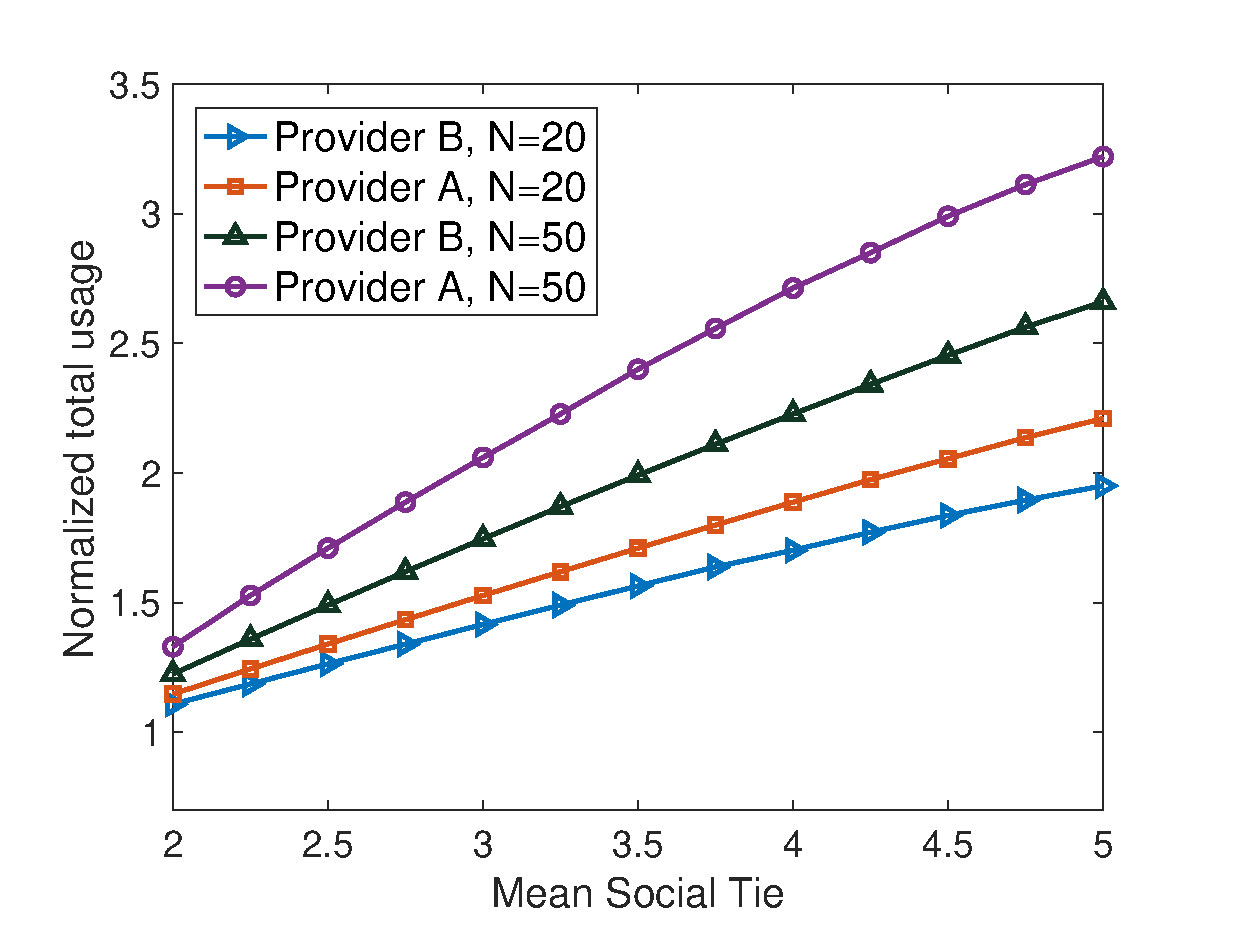
\includegraphics[scale=0.53]{./pic/normusage2.eps}
\vspace{-0.0cm}
%\caption{Impact of mean of social tie $\mu_{G}$ on total data usage.}\label{fg:Fig1}
\caption{社交联结权值平均值$\mu_{G}$对总数据使用量的影响。}\label{fg:Fig1}
\end{figure}

\begin{figure}[htb]
\centering
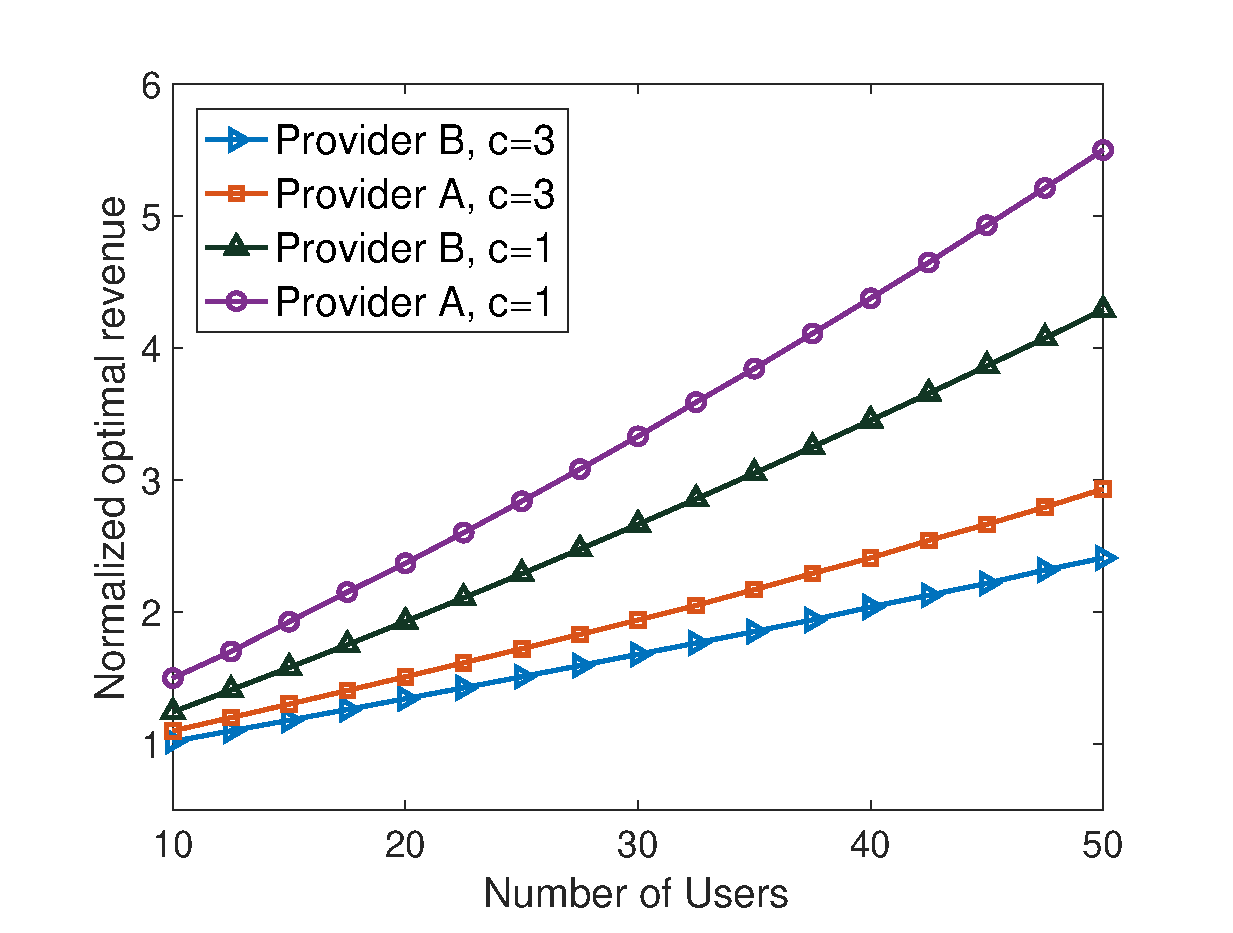
\includegraphics[scale=0.53]{./pic/normrev2.eps}
\vspace{-0.0cm}
%\caption{Normalized optimal revenue versus number of users $N$.}\label{fg:Fig2}
\caption{归一化最佳收益与用户数量$N$变化关系。}\label{fg:Fig2}
\end{figure}

\begin{figure}[htb]
\centering
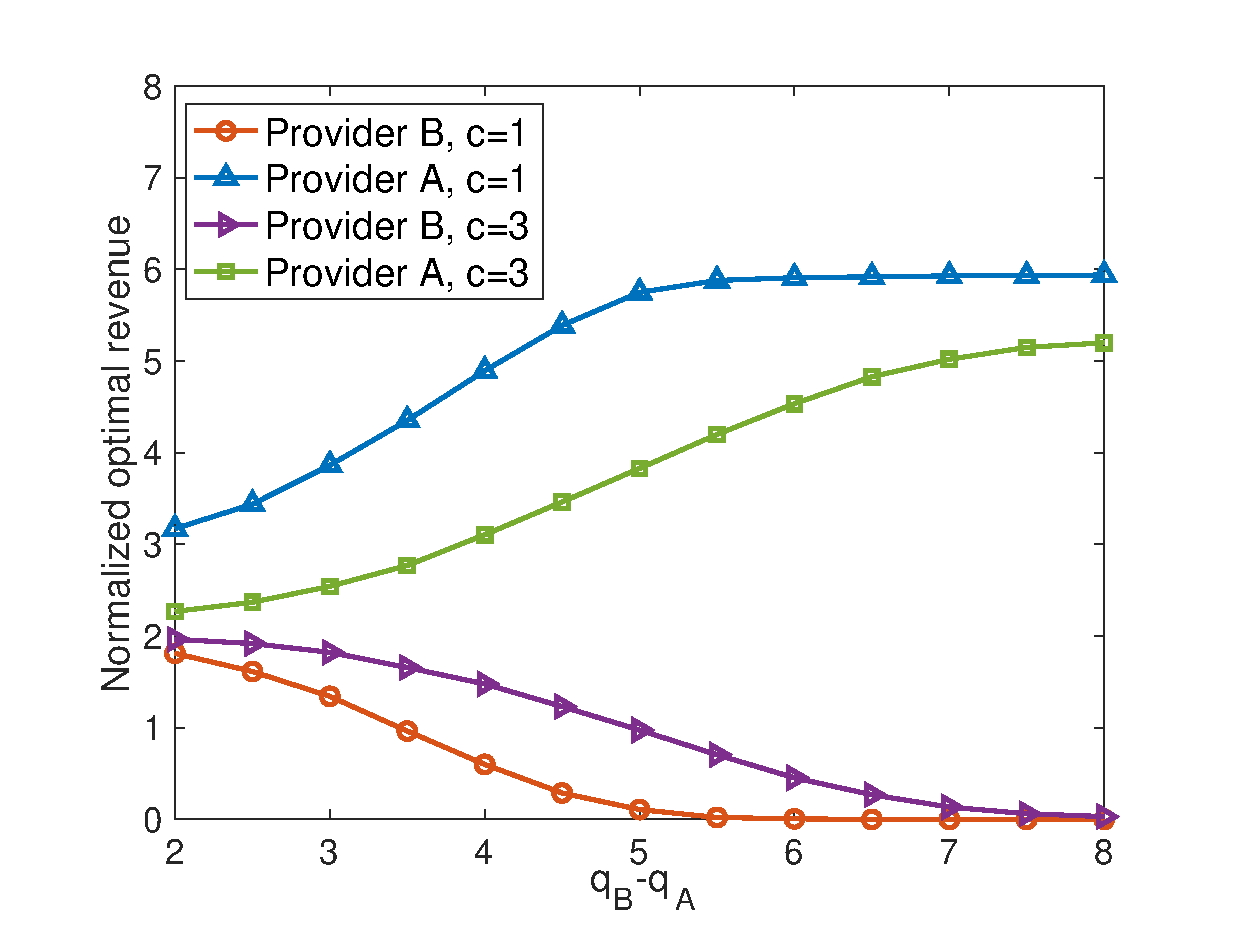
\includegraphics[scale=0.53]{./pic/cost2.eps}
\vspace{-0.0cm}
%\caption{Normalized optimal revenue versus service cost difference.}\label{fg:Fig3}
\caption{归一化的最佳收益与服务成本差异之间的关系。}\label{fg:Fig3}
\end{figure}

\begin{figure}[htb]
\centering
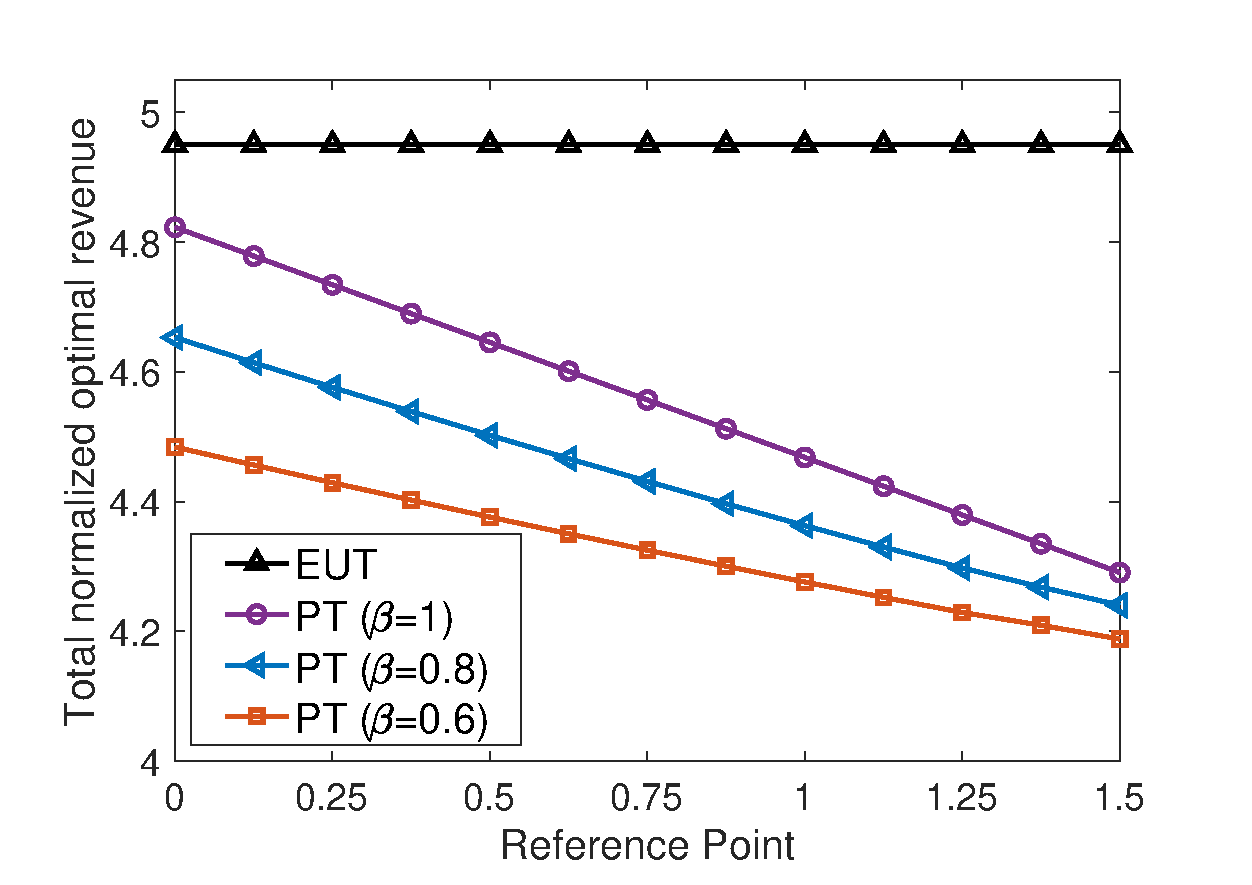
\includegraphics[scale=0.53]{./pic/prospect2.eps}
\vspace{-0.0cm}
%\caption{Impact of bounded rationality on service providers' total revenue.}\label{fg:prospect}
\caption{有限理性对服务提供商总收益的影响。}\label{fg:prospect}
\end{figure}

我们首先考虑理性服务提供商的情况,来模拟服务商定价-用户数据使用博弈,并设置参数$\epsilon=0.4$。为了评估在均衡状态下网络外部性对用户数据使用的影响,我们分别针对拥有20个用户的市场和拥有50个用户的市场两种情况,将拥塞系数固定在默认值,同时将社交联结权值均值$\mu_{G}$从2增加到5。图\ref{fg:Fig1}说明了移动用户的数据总使用量随$\mu_{G}$取值增加而单调增加;对于50个用户的情况,数据使用量整体上更多。该结果清楚地表明,通过加强社交联系以增强正网络外部性效应可以推动移动用户从服务提供商那里消费更多数据。
%We first consider the scenario with rational service providers and simulate the pricing-usage game using the algorithm proposed in our previous paper \cite{MYCISS16}, with parameter $\epsilon$ set to be 0.4. To evaluate the impact of enhancing network effect on users' data usage at equilibrium, we increase the mean social tie strength $\mu_{G}$ from 2 to 5, for a market with 20 users and one with 50 users respectively, letting the congestion coefficient being set as default. Fig. \ref{fg:Fig1} illustrates that mobile users' normalized total usage increases monotonically with $\mu_{G}$, and the normalized total usage is greater for the case with 50 users. This result clearly demonstrates that strengthened social connections, hence a stronger network effect, can push the mobile users to consume more data from service providers.

接下来,我们分析评估无线服务提供商可实现的收益。我们将平均社会联结强度固定为$\mu_{G}=2$,并针对轻度拥塞($c=1$)和重度拥塞($c=3$)分别将系统用户数量从10增加到50两种情况进行仿真。如图\ref{fg:Fig2}所示,服务提供商在均衡状态下的标准化收益随市场规模的增加而单调增加。而且正如预期的那样,当系统自身拥塞情况较轻微时,服务提供商将获得更高的收益。
%We then turn to evaluate the attainable revenues for the wireless service providers. We fix the mean social tie strength as $\mu_{G}=2$ and simulate the system with user amount changing from 10 to 50, for both a light congestion scheme ($c=1$) and a heavy congestion scheme ($c=3$). As illustrated in Fig. \ref{fg:Fig2}, the service providers' normalized revenues at equilibrium increase monotonically as the size of market increases. Also, as expected, service providers receive higher revenues when the congestion level is lower. 

我们进一步评估服务提供商之间的竞争对其各自收益的影响。我们令$q_{a}=1$将$q_{b}$的值从3改变到9,从而使得服务成本差异从2增长到8(提供商$A$相比提供商$B$在服务成本上更具竞争力)。如图\ref{fg:Fig3}所示,随着成本差异的扩大,服务提供商$A$的收益不断增加,而提供商$B$的收益却不断下降。当达到一定成本差异时,提供商$B $的收入减少到零,并且提供商$A$的收益趋于饱和,这意味着所有用户都选择使用服务提供商$A$的数据。
%We next evaluate the impact on the normalized revenues from the competition between the two service providers. We set $q_{a}=1$ and changed $q_{b}$ from 3 to 9 so that the service cost difference was altered from 2 to 8 (provider $A$ is more competitive compared to provider $B$ in terms of the service cost). As illustrated in Fig. \ref{fg:Fig3}, with the enlarging cost difference, service provider $A$ has an increasing normalized revenue while the revenue of provider $B$ keeps decreasing. At a certain level of cost difference, the revenue of provider $B$ diminishes to zero and the revenue of provider $A$ becomes saturated, which means that all users choose to consume data from service provider $A$. 

最后,我们通过比较PT模型下的最优收益与传统EUT模型下的最优收益,来分析服务提供商行为理性的影响。对于PT模型,在仿真中我们为两个服务提供商选择相同的参考点和风险规避参数(即$R_A=R_B= R$,$\beta_A=\beta_B=\beta$)。我们进一步设置概率失真参数$\alpha=0.6$和损失惩罚参数$\lambda=1.5$。对于分布式学习算法,我们设置学习参数$\theta^t=1/t$,温度参数$\eta=5$。我们为风险规避参数选择三个不同的值(即$\beta=1,0.8,0.6$),然后对于$R$取值在0到3的范围内进行仿真。如图\ref{fg:prospect}所示,总收益会随着参考点取值的增加而减少。从本质上讲,参考点取值偏离零值越多,将导致服务提供商的客观评估发生更大的偏移,从而使他们对收益增益的重视程度降低,而对收益损失的重视程度更高。此外,较小的$\beta$值会导致收益进一步下降,因为当服务提供商风险规避程度增加时,等量收益增益对于提供商的价值会降低。通过设置$\beta=1$,我们移除了参数$\beta$的影响;在$R=0$处EUT曲线和PT曲线之间的间隙表示近由于概率失真效应而导致的收入下降。
%At last, we investigate the impact of rationality of service providers by comparing the optimal revenue under the PT model (via using Algorithm 1) to the one under the conventional EUT model. For the case with PT model, we choose the same reference point and utility aversion parameter for both service providers (i.e., $R_A=R_B=R$, $\beta_A=\beta_B=\beta$). We further set the probability distortion parameter $\alpha=0.6$ and the loss penalty parameter $\lambda=1.5$. For the distributed learning algorithm, we set the learning parameter $\theta^t=1/t$, and the temperature parameter $\eta=5$. We choose three different values for the utility aversion parameters (i.e., $\beta=1, 0.8, 0.6$), and run the simulation with $R$ increasing from 0 to 3. As illustrated in Fig. \ref{fg:prospect}, the total revenue decreases as the reference point increases. In essence, a larger reference point will lead to a greater shift of service providers' objective evaluation, so that they value less on their gain but more on their loss. In addition, a smaller value of $\beta$ leads to further degradation of revenue since service providers value their gain less when they become more gain-averse. It is also shown that the degradation due to smaller $\beta$ reduces as the reference point increases. We eliminate the impact of parameter $\beta$ by setting $\beta=1$; the gap between the EUT curve and PT curve at $R=0$ indicates the revenue degradation solely due to the probability distortion effect.

\section{本章小结}\label{sec:tvtcon}
在本文中,我们探讨了在社交效应与拥塞效应形成的双重网络外部性影响下无线服务提供商的定价策略和移动用户的数据消费行为。为了刻画移动用户和服务提供商之间的交互,我们使用了斯塔克伯格博弈的问题建模并分析了其均衡解。特别地,我们首先求解了博弈第二阶段的链接需求均衡,并证明了博弈均衡的唯一性特征。接着我们分别在传统的完全理性服务提供商场景和更实际的有限理性服务提供商场景下证明了第二阶段中混合策略定价均衡的存在。我们的数值结果体现了社交效应和拥塞效应对系统性能的影响,以及有限理性行为对服务提供商收入造成的负面影响。
%In this paper, we explored the wireless service providers' pricing strategies and mobile users' data consumption behavior. To characterize the interactions between mobile users and service providers, we appealed to the Stackelberg game model and analyzed its equilibrium solution. Particularly, we first solved the link demand equilibrium in Stage II of the game and showed its uniqueness property. We then established the existence of a mixed-strategy pricing equilibrium in Stage I, under both the conventional scenario with rational service providers and the more realistic scenario with bounded rational providers. Our numerical results provide insight on the impact of positive network effect and congestion effect over the system performance, as well as the negative influence on service providers' revenues caused by their bounded rational behavior.

%在以后的工作中,我们将考虑使用替代模型来更好地描述拥塞效应。另一个未来的方向是进行一些基于真实数据的实验,以验证网络效应和拥塞效应对系统性能的影响。
%For future work, we will consider alternative model to better characterize the congestion effect. Another future direction is to conduct some real-data based experiment to verify the impacts of network effect and congestion effect on the system performance.
